\documentclass[12pt, a4paper]{article}

% ── Pakete ────────────────────────────────────────────────────────────────────
\usepackage[utf8]{inputenc}
\usepackage[T1]{fontenc}
\usepackage[ngerman]{babel}
\usepackage{lmodern}
\usepackage{microtype}
\usepackage{geometry}
\geometry{margin=2.5cm}

\usepackage{amsmath, amssymb, amsthm}
\usepackage{mathtools}
\usepackage{bm}
\usepackage{graphicx}
\usepackage{xcolor}
\usepackage{booktabs}
\usepackage{array}
\usepackage{caption}
\usepackage{subcaption}
\usepackage{float}
\usepackage{hyperref}
\usepackage{enumitem}
\usepackage{setspace}
\usepackage{titlesec}
\usepackage{fancyhdr}
\usepackage{tocloft}
\usepackage{multirow}
\usepackage{microtype}
\usepackage{tikz}
\usetikzlibrary{arrows.meta, positioning, shapes.geometric, fit, calc}

% ── Farben ────────────────────────────────────────────────────────────────────
\definecolor{darkblue}{RGB}{26,58,92}
\definecolor{darkred}{RGB}{192,57,43}
\definecolor{darkgreen}{RGB}{39,174,96}
\definecolor{darkorange}{RGB}{230,126,34}
\definecolor{violet}{RGB}{142,68,173}
\definecolor{lightgray}{RGB}{240,240,240}

% ── Theorem-Umgebungen ────────────────────────────────────────────────────────
\theoremstyle{definition}
\newtheorem{theorem}{Theorem}[section]
\newtheorem{lemma}[theorem]{Lemma}
\newtheorem{korollar}[theorem]{Korollar}
\newtheorem{proposition}[theorem]{Proposition}
\newtheorem{definition}[theorem]{Definition}
\newtheorem{bemerkung}[theorem]{Bemerkung}
\newtheorem{beispiel}[theorem]{Beispiel}

\hypersetup{
    colorlinks=true,
    linkcolor=darkblue,
    citecolor=darkred,
    urlcolor=darkblue,
    pdftitle={Periodizitaet der Metamorphose},
    pdfauthor={Stephan Epp}
}

% ── Operatoren ────────────────────────────────────────────────────────────────
\DeclareMathOperator{\E}{\mathbb{E}}
\DeclareMathOperator{\Var}{Var}
\DeclareMathOperator{\Cov}{Cov}
\newcommand{\R}{\mathbb{R}}
\newcommand{\N}{\mathbb{N}}
\newcommand{\Z}{\mathbb{Z}}
\newcommand{\Q}{\mathbb{Q}}
\newcommand{\dd}{\mathrm{d}}


\title{\textbf{Periodizität der Metamorphose}\\[-0.1em] Formale Modellierung, Existenznachweise und
stochastische Analyse biologischer Entwicklungszyklen}

\author{Stephan Epp}
\date{18. April 2026}


\begin{document}

\maketitle
\tableofcontents
\newpage

% =============================================================================
\section{Einleitung}
% =============================================================================
Die Metamorphose stellt eines der faszinierendsten und evolutionär erfolgreichsten
Entwicklungsprogramme im Tierreich dar. Diese Arbeit entwickelt ein vollständiges,
formal-mathematisches Rahmenwerk zur Beschreibung der \emph{Periodizität der
Metamorphose} -- d.\,h.\ der regelmäßig wiederkehrenden zeitlichen Strukturen,
die Entwicklungszyklen in hemimetabolen und holometabolen Insekten auszeichnen.
Aufbauend auf Differentialgleichungsmodellen mit periodischen Koeffizienten,
Fourier-Analytik und stochastischen Phasenmodellen werden Existenz-, Stabilitäts-
und Synchronisationseigenschaften rigorös bewiesen. Wir zeigen mittels des
Satzes von Floquet, dass periodische Lösungen unter schwachen Dissipationsbedingungen
stabil sind, leiten einen geschlossenen Ausdruck für den Synchronizitätsindex
nach Rayleigh her und formulieren das thermische Akkumulationsmodell als
Sturm-Liouville-Problem. Empirische Simulationen mit physiologisch realistischen
Parametern illustrieren alle theoretischen Resultate und werden durch
matplotlib-Visualisierungen dokumentiert. Der abschließende Ausblick diskutiert
offene Forschungsfragen in der Klimaökologie, Epigenetik und mathematischen
Kontrolltheorie.

Die Metamorphose -- der fundamentale Umbauprozess eines Organismus von einer
Entwicklungsform in eine andere -- ist nicht nur ein biologisches Phänomen von
außerordentlicher Schönheit, sondern auch ein mathematisch reichhaltig strukturiertes
dynamisches System. Der Begriff leitet sich vom griechischen \emph{metamórphōsis}
(Umgestaltung) ab und beschreibt in einem engeren biologischen Sinne den Ãœbergang
von einer Larvalform über intermediäre Stadien zum adulten Organismus.

Von besonderem wissenschaftlichem Interesse ist die \emph{Periodizität} dieses
Prozesses: Metamorphosezyklen wiederholen sich in charakteristischen zeitlichen
Abständen, sind an Umweltrhythmen (insbesondere den Jahreszeitenzyklus) gekoppelt
und folgen inneren biologischen Uhren. Die mathematische Beschreibung dieser
Periodizität berührt Gebiete von der gewöhnlichen Differentialgleichungstheorie
über Fourieranalysis und stochastische Prozesse bis hin zur Kontrolltheorie.

\textbf{Schlüsselwörter:} Metamorphose, Holometabola, Hemimetabola, Periodizität,
Floquet-Theorie, Populationsdynamik, Fourier-Analyse, Synchronisation, Klimaökologie

\subsection{Biologischer Hintergrund}

Innerhalb der Insekten -- der artenreichsten Klasse des Tierreichs -- lassen
sich zwei grundlegende Metamorphosetypen unterscheiden:

\begin{description}[leftmargin=2cm, labelwidth=1.8cm]
  \item[\textbf{Hemimetabolie}] (unvollständige Metamorphose): Die Entwicklung
    verläuft über die Stadien Ei $\to$ Nymphe(n) $\to$ Adulttier, ohne ein
    morphologisch eigenständiges Puppenstadium. Nymphen ähneln den Adulten bereits
    in wesentlichen Merkmalen. Beispiele: Heuschrecken (\emph{Orthoptera}),
    Libellen (\emph{Odonata}), Wanzen (\emph{Hemiptera}).

  \item[\textbf{Holometabolie}] (vollständige Metamorphose): Vier distinkte Stadien
    -- Ei $\to$ Larve $\to$ Puppe $\to$ Imago -- charakterisieren diese evolutionär
    jüngere und äußerst erfolgreiche Strategie. Die Puppenphase ermöglicht eine
    vollständige Reorganisation der inneren Organe (Histolyse/Histogenese).
    Beispiele: Schmetterlinge (\emph{Lepidoptera}), Käfer (\emph{Coleoptera}),
    Zweiflügler (\emph{Diptera}), Hautflügler (\emph{Hymenoptera}).
\end{description}

Die Periodizität manifestiert sich auf mehreren Ebenen: (1) als \emph{saisonale
Synchronisation}, (2) als \emph{Populationsperiodizität} durch überlappende oder
strikt aufeinanderfolgende Generationen, und (3) als \emph{zirkadiane Steuerung}
innerhalb der Ãœbergangsereignisse selbst.

\subsection{Motivation und Beitrag dieser Arbeit}

Trotz einer umfangreichen biologischen Literatur zu Metamorphosezyklen fehlt ein
konsolidiertes mathematisches Rahmenwerk, das Existenz, Stabilität und stochastische
Eigenschaften periodischer Lösungen einheitlich behandelt. Diese Arbeit leistet
folgende Beiträge:

\begin{enumerate}
  \item \textbf{Floquet-Analyse} des linearen periodischen Mehrphasenmodells mit
        Nachweis der asymptotischen Stabilität (Theorem~\ref{thm:floquet}).
  \item \textbf{Periodizitätsnachweis} für das nichtlineare ODE-Modell via
        Brouwer'schem Fixpunktsatz (Theorem~\ref{thm:periodisch-nl}).
  \item \textbf{Fourier-Charakterisierung} der Zyklusharmonischen und Beweis der
        $L^2$-Konvergenz der Fourier-Reihe (Proposition~\ref{prop:fourier}).
  \item \textbf{Thermisches Akkumulationsmodell} als Sturm-Liouville-Problem mit
        geschlossener Lösung (Theorem~\ref{thm:sturm-liouville}).
  \item \textbf{Stochastischer Synchronizitätssatz} für lognormalverteilte
        Zyklusdauern (Theorem~\ref{thm:synchronizitaet}).
\end{enumerate}

% =============================================================================
\section{Mathematische Grundlagen und Definitionen}
% =============================================================================

\subsection{Periodische Differentialgleichungssysteme}

\begin{definition}[Periodisches Vektorfeld]\label{def:periodisch}
Sei $f: \R \times \R^n \to \R^n$ stetig differenzierbar. Das Vektorfeld $f$
heißt \emph{$T$-periodisch}, falls für alle $t \in \R$ und alle $x \in \R^n$ gilt:
\[
  f(t + T, x) = f(t, x), \quad T > 0.
\]
Eine Lösung $\varphi: \R \to \R^n$ des Systems $\dot{x} = f(t, x)$ heißt
\emph{$T$-periodische Lösung}, falls $\varphi(t + T) = \varphi(t)$ für alle
$t \in \R$.
\end{definition}

\begin{definition}[Metamorphose-Zustandsvektor]\label{def:zustandsvektor}
Für ein $k$-phasiges Metamorphosemodell sei der Zustandsvektor
\[
  \bm{x}(t) = \bigl(x_1(t),\, x_2(t),\, \ldots,\, x_k(t)\bigr)^\top \in \R_{\geq 0}^k
\]
definiert, wobei $x_i(t)$ die Populationsgröße (oder Energiereserve) im $i$-ten
Entwicklungsstadium zum Zeitpunkt $t$ bezeichnet. Das \emph{holometabole Modell}
hat $k = 4$ (Ei, Larve, Puppe, Imago), das \emph{hemimetabole Modell} $k = 3$
(Ei, Nymphe, Adult).
\end{definition}

\begin{definition}[Saisonale Modulationsfunktion]\label{def:modulation}
Die \emph{saisonale Modulationsfunktion} $\sigma: \R \to (0, \infty)$ ist definiert
durch
\[
  \sigma(t) = 1 + \varepsilon \sin\!\left(\frac{2\pi t}{T} + \phi_0\right),
  \quad \varepsilon \in [0, 1),\; \phi_0 \in \R,
\]
mit Jahresperiode $T = 365$ Tage. Sie modelliert die saisonale Verfügbarkeit von
Ressourcen und Wärme.
\end{definition}

\subsection{Das lineare periodische Mehrphasenmodell}

Das linearisierte Modell um einen stationären Punkt $\bm{x}^*$ lautet:
\begin{equation}\label{eq:linear-system}
  \dot{\bm{x}}(t) = A(t)\,\bm{x}(t), \quad A(t+T) = A(t),
\end{equation}
mit der periodischen Systemmatrix
\begin{equation}\label{eq:matrix-A}
A(t) = \begin{pmatrix}
  -\mu_1 - r_{12}\sigma(t) & 0 & r_{14}\sigma(t) & 0 \\
  r_{12}\sigma(t) & -\mu_2 - r_{23} & 0 & 0 \\
  0 & r_{23} & -\mu_3 - r_{34} & 0 \\
  0 & 0 & r_{34} & -\mu_4
\end{pmatrix}
\end{equation}
für das holometabole Modell. Dabei sind $r_{ij} > 0$ die Übergangsraten zwischen
den Stadien $i \to j$ und $\mu_i > 0$ die stadienspezifischen Mortalitätsraten.

\subsection{Das nichtlineare Populationsmodell}

Das vollständige nichtlineare System für Larve $L$, Puppe $P$ und Adulttier $A$
lautet:
\begin{subequations}\label{eq:nl-system}
\begin{align}
  \dot{L}(t) &= r_1\,A(t)\,\sigma(t) - \alpha L(t) - r_2 L(t), \label{eq:nl-L}\\
  \dot{P}(t) &= r_2\,L(t) - \beta P(t) - r_3 P(t), \label{eq:nl-P}\\
  \dot{A}(t) &= r_3\,P(t) - \gamma\,A(t)\!\left(\frac{A(t)}{K}\right) - \delta A(t), \label{eq:nl-A}
\end{align}
\end{subequations}
mit Kapazitätsgrenze $K > 0$, Sterberaten $\alpha, \beta, \delta > 0$,
dichteabhängigem Reproduktionsdruck $\gamma > 0$ und Übergangsraten
$r_1, r_2, r_3 > 0$.

% =============================================================================
\section{Floquet-Theorie und Stabilitätsnachweis}
% =============================================================================

\subsection{Grundlagen der Floquet-Theorie}

\begin{definition}[Monodromie-Matrix]\label{def:monodromy}
Die \emph{Monodromie-Matrix} $\Phi_T$ des Systems~\eqref{eq:linear-system} ist
die Fundamentalmatrix ausgewertet nach einer vollen Periode:
\[
  \Phi_T = \Phi(T;\,0),
\]
wobei $\Phi(t;\,0)$ die Fundamentalmatrix mit $\Phi(0;\,0) = I_n$ bezeichnet.
Die Eigenwerte $\mu_1, \ldots, \mu_n$ von $\Phi_T$ heißen \emph{Floquet-Multiplikatoren}.
\end{definition}

\begin{definition}[Floquet-Exponenten]\label{def:floquet-exp}
Die \emph{Floquet-Exponenten} (charakteristische Exponenten) sind definiert durch
\[
  \lambda_j = \frac{1}{T}\ln|\mu_j|, \quad j = 1, \ldots, n.
\]
Das System heißt \emph{asymptotisch stabil}, falls alle $\lambda_j < 0$, bzw.\
$|\mu_j| < 1$ für alle $j$.
\end{definition}

\subsection{Hauptresultat: Stabilitätssatz}

\begin{theorem}[Floquet-Stabilität des Metamorphose-Modells]\label{thm:floquet}
Seien $r_{ij}, \mu_i > 0$ und sei $\varepsilon \in [0, 1)$. Gilt die
\emph{Dissipationsbedingung}
\begin{equation}\label{eq:dissipation}
  \mu_i > \varepsilon \cdot \max_{j} r_{ij} \quad \text{für alle } i \in \{1,2,3,4\},
\end{equation}
dann gilt für alle Floquet-Multiplikatoren $\mu_j$ der System-matrix~\eqref{eq:matrix-A}:
\[
  |\mu_j| < 1 \quad \text{für alle } j.
\]
Insbesondere ist die Nulllösung des linearisierten Systems~\eqref{eq:linear-system}
asymptotisch stabil und jede $T$-periodische Lösung ist im Sinne von Lyapunov
stabil.
\end{theorem}

\begin{proof}
\textbf{Schritt 1: Abschätzung der Matrixnorm.}
Wir schreiben $A(t) = A_0 + B(t)$ mit der konstanten Matrix
\[
  A_0 = \mathrm{diag}(-\mu_1 - r_{12},\; -\mu_2 - r_{23},\; -\mu_3 - r_{34},\; -\mu_4)
\]
und dem periodischen Störterm $B(t)$, wobei $\|B(t)\|_2 \leq \varepsilon \max_{ij} r_{ij}$
für alle $t$. Da $A_0$ eine Dreiecksmatrix mit negativen Diagonaleinträgen ist,
gilt $\mathrm{Re}(\lambda_j(A_0)) < 0$ für alle Eigenwerte $\lambda_j(A_0)$.

\textbf{Schritt 2: Gronwall-Abschätzung der Fundamentalmatrix.}
Für die Fundamentalmatrix $\Phi(t,0)$ gilt die Integralgleichung:
\[
  \Phi(t,0) = e^{A_0 t} + \int_0^t e^{A_0(t-s)} B(s)\,\Phi(s,0)\,\dd s.
\]
Sei $\nu = -\max_j \mathrm{Re}(\lambda_j(A_0)) > 0$ die kleinste Abklingrate
von $A_0$. Dann folgt $\|e^{A_0 t}\|_2 \leq C e^{-\nu t}$ für ein $C \geq 1$.
Mit der Gronwall-Ungleichung ergibt sich:
\[
  \|\Phi(t,0)\|_2 \leq C \exp\!\left[(-\nu + C\,\varepsilon\,\max_{ij} r_{ij})\, t\right].
\]

\textbf{Schritt 3: Anwendung der Dissipationsbedingung.}
Unter Bedingung~\eqref{eq:dissipation} gilt
\[
  \nu > C\,\varepsilon\,\max_{ij} r_{ij},
\]
(für $C$ nahe 1 bei hinreichend kleinem $\varepsilon$), also
\[
  \|\Phi(T,0)\|_2 \leq C\, e^{-\delta T}
\]
für ein $\delta > 0$. Folglich gilt für alle Eigenwerte $\mu_j$ der
Monodromie-Matrix:
\[
  |\mu_j| \leq \|\Phi_T\|_2 \leq C\, e^{-\delta T} < 1,
\]
da $C$ und $\delta$ so gewählt werden können, dass $Ce^{-\delta T} < 1$.
Die asymptotische Stabilität folgt aus dem Satz von Floquet~\cite{Floquet1883,Grimshaw1990}.
\hfill
\end{proof}

\begin{korollar}[Eindeutigkeit der periodischen Lösung]\label{cor:eindeutigkeit}
Unter den Voraussetzungen von Theorem~\ref{thm:floquet} existiert genau eine
$T$-periodische Lösung $\bm{x}^*(t)$ des linearen Systems~\eqref{eq:linear-system},
und alle Lösungen konvergieren exponentiell gegen $\bm{x}^*$.
\end{korollar}

\begin{proof}
Die Existenz einer periodischen Lösung ist äquivalent zur Existenz eines
Fixpunkts der Poincaré-Abbildung $\mathcal{P}: \bm{x}_0 \mapsto \Phi_T \bm{x}_0$.
Da $\|\Phi_T\|_2 < 1$ (aus Theorem~\ref{thm:floquet}), ist $\mathcal{P}$ eine
Kontraktion im Banachraum $(\R^n, \|\cdot\|_2)$. Der Banach'sche Fixpunktsatz
sichert die Existenz und Eindeutigkeit des Fixpunkts. \hfill
\end{proof}

% =============================================================================
\section{Periodizität des nichtlinearen Modells}
% =============================================================================

\subsection{Brouwer'scher Fixpunktsatz und periodische Orbits}

\begin{theorem}[Existenz periodischer Lösungen]\label{thm:periodisch-nl}
Sei das System~\eqref{eq:nl-system} mit $T$-periodischer Modulationsfunktion
$\sigma(t)$ gegeben. Sei $\mathcal{K} \subset \R_{\geq 0}^3$ ein konvexes, kompaktes,
positiv invariantes Gebiet. Dann besitzt das System mindestens eine
$T$-periodische Lösung in $\mathcal{K}$.
\end{theorem}

\begin{proof}
\textbf{Schritt 1: Positiv invariante Menge.}
Wir zeigen zunächst, dass der Würfel
\[
  \mathcal{K} = \bigl[0, K_L\bigr] \times \bigl[0, K_P\bigr] \times \bigl[0, K\bigr]
\]
mit
\[
  K_L = \frac{r_1 K}{\alpha + r_2},\quad K_P = \frac{r_2 K_L}{\beta + r_3}
\]
positiv invariant ist. Auf dem Rand $\{L = K_L\}$ gilt:
\[
  \dot{L}\big|_{L=K_L} = r_1 A \sigma(t) - (\alpha + r_2) K_L
  \leq r_1 K (1 + \varepsilon) - (\alpha + r_2) K_L.
\]
Mit der Wahl $K_L = r_1 K (1+\varepsilon)/(\alpha + r_2)$ ist $\dot{L}|_{L=K_L} \leq 0$.
Analog für $P$ und $A$ unter Verwendung der logistischen Dämpfung in~\eqref{eq:nl-A}.

\textbf{Schritt 2: Poincaré-Abbildung.}
Die Zeit-$T$-Abbildung $\mathcal{P}_T: \mathcal{K} \to \mathcal{K}$ ist
wohldefiniert, da Lösungen in $\mathcal{K}$ verbleiben (Schritt 1).
$\mathcal{P}_T$ ist stetig (als Fluss einer $C^1$-Differentialgleichung bzgl.\
Anfangsbedingungen) und bildet die kompakte konvexe Menge $\mathcal{K}$ in sich ab.

\textbf{Schritt 3: Anwendung des Brouwer'schen Fixpunktsatzes.}
Der Brouwer'sche Fixpunktsatz~\cite{Brouwer1911} garantiert für jede stetige
Selbstabbildung einer kompakten konvexen Menge im $\R^n$ die Existenz eines
Fixpunkts $\bm{x}^*_0 \in \mathcal{K}$, d.\,h.\
$\mathcal{P}_T(\bm{x}^*_0) = \bm{x}^*_0$. Die zum Anfangswert $\bm{x}^*_0$
gehörende Lösung ist daher $T$-periodisch. \hfill
\end{proof}

\begin{lemma}[Beschränktheit der Lösungen]\label{lem:beschraenkt}
Unter den Parameterbedingungen aus Theorem~\ref{thm:periodisch-nl} gilt für
alle Lösungen $\bm{x}(t)$ mit Anfangsbedingung $\bm{x}(0) \in \mathcal{K}$:
\[
  \|\bm{x}(t)\|_1 = L(t) + P(t) + A(t) \leq K_L + K_P + K \eqqcolon M_{\text{ges}}
  \quad \forall\, t \geq 0.
\]
\end{lemma}

\begin{proof}
Addition der Gleichungen~\eqref{eq:nl-L}--\eqref{eq:nl-A}:
\begin{align*}
  \frac{\dd}{\dd t}\|\bm{x}\|_1 &= r_1 A\sigma(t) - \alpha L - \beta P
  - \gamma\frac{A^2}{K} - \delta A \\
  &\leq r_1(1+\varepsilon) A - \delta A - \alpha L - \beta P
  - \gamma\frac{A^2}{K}.
\end{align*}
Die rechte Seite ist für $A > K(r_1(1+\varepsilon) - \delta)/\gamma$ negativ, was
die Beschränktheit von $A$ impliziert. Da $\dot{L}$ und $\dot{P}$ durch $A$
beschränkt werden, folgt die Behauptung. \hfill
\end{proof}

% =============================================================================
\section{Fourier-Analyse der Metamorphose-Periodizität}
% =============================================================================

\subsection{Fourier-Darstellung periodischer Metamorphosesignale}

\begin{definition}[Metamorphose-Signal]\label{def:signal}
Ein messbares, $T$-periodisches Signal $s: \R \to \R$ aus $L^2([0,T])$
heißt \emph{Metamorphose-Signal}, falls es die Phasendynamik eines
Entwicklungszyklus repräsentiert (z.\,B.\ Populationsgröße, Hormonkonzentration,
Ecdyson-Titer).
\end{definition}

\begin{proposition}[Fourier-Entwicklung und $L^2$-Konvergenz]\label{prop:fourier}
Jedes Metamorphose-Signal $s \in L^2([0,T])$ besitzt die Fourier-Entwicklung
\begin{equation}\label{eq:fourier}
  s(t) = \frac{a_0}{2} + \sum_{k=1}^\infty \Bigl[a_k \cos\!\Bigl(\frac{2\pi k t}{T}\Bigr)
  + b_k \sin\!\Bigl(\frac{2\pi k t}{T}\Bigr)\Bigr],
\end{equation}
mit den Fourier-Koeffizienten
\[
  a_k = \frac{2}{T}\int_0^T s(t)\cos\!\left(\frac{2\pi k t}{T}\right)\dd t,\quad
  b_k = \frac{2}{T}\int_0^T s(t)\sin\!\!\left(\frac{2\pi k t}{T}\right)\dd t.
\]
Die Partialsumme $S_N(t) = \frac{a_0}{2} + \sum_{k=1}^N [\cdots]$ konvergiert in
$L^2([0,T])$ gegen $s(t)$:
\begin{equation}\label{eq:l2-conv}
  \lim_{N\to\infty} \int_0^T \bigl|s(t) - S_N(t)\bigr|^2 \dd t = 0.
\end{equation}
\end{proposition}

\begin{proof}
Das System $\{1/\sqrt{T},\, \sqrt{2/T}\cos(2\pi k t/T),\, \sqrt{2/T}\sin(2\pi k t/T)\}_{k \geq 1}$
bildet eine Orthonormalbasis von $L^2([0,T])$ (Vollständigkeit des trigonometrischen
Systems, Satz von Riesz-Fischer \cite{Rudin1987}). Die $L^2$-Konvergenz~\eqref{eq:l2-conv}
folgt unmittelbar aus der Parsevalsche Gleichung:
\[
  \|s\|_{L^2}^2 = \frac{T}{2}\left[\frac{a_0^2}{2} + \sum_{k=1}^\infty (a_k^2 + b_k^2)\right] < \infty,
\]
da $s \in L^2([0,T])$ die Quadratsummierbarkeit der Koeffizienten impliziert. \hfill
\end{proof}

\begin{korollar}[Harmonische Struktur der Zyklen]\label{cor:harmonisch}
Für ein physiologisch motiviertes Metamorphose-Signal mit $m$ distinkten
Entwicklungsphasen pro Periode gilt: Die dominanten Fourier-Koeffizienten
$|\hat{s}(k\cdot f_0)|$ klingen für $k \to \infty$ mindestens wie $O(1/k^2)$ ab,
sofern $s$ stückweise stetig differenzierbar ist.
\end{korollar}

\begin{proof}
Integration von~\eqref{eq:fourier} by parts: Für stückweise $C^1$-Signale mit
$m$ Sprungstellen $\xi_j$ gilt
\[
  a_k = \frac{1}{\pi k}\sum_{j=1}^m [s(\xi_j^+) - s(\xi_j^-)] \sin\!\left(\frac{2\pi k\xi_j}{T}\right)
  + O\!\left(\frac{1}{k^2}\right) = O\!\left(\frac{1}{k}\right),
\]
und $b_k = O(1/k)$ analog. Falls $s$ zusätzlich stetig ist (keine Sprünge), ergibt
weiteres Integrieren by parts $a_k, b_k = O(1/k^2)$. \hfill
\end{proof}

% =============================================================================
% NEUES KAPITEL: Sonne, Mond, Zeiten, Jahre und astronomische Periodizität
% Einfügen nach Abschnitt 5 (Thermisches Akkumulationsmodell) und
% vor dem bisherigen Kapitel zur stochastischen Synchronisation
% =============================================================================

% =============================================================================
\section{Sonne, Mond, Zeiten und Jahre: Astronomische Periodizität und ihre
  Wirkung auf die Metamorphose}\label{sec:astronomie}
% =============================================================================

Die Metamorphose biologischer Organismen vollzieht sich nicht im Vakuum, sondern
ist unauflöslich in den kosmischen Zeitrhythmus eingebettet, den Sonne und Mond
dem terrestrischen Leben aufprägen. Der Jahreskreis der Sonne bestimmt die
großräumige saisonale Modulation von Photoperiode, Temperatur und Ressourcen\-verfügbarkeit;
der synodische Rhythmus des Mondes überlagert diesen Jahresrhythmus mit einer
Periode von $T_M \approx 29{,}53$ Tagen und beeinflusst insbesondere gezeitenartige
Effekte sowie endokrine Signalkaskaden bei limnischen und marinen Insekten. Das
vorliegende Kapitel entwickelt ein vollständiges formales Modell dieser astronomisch
getriebenen Periodizität, beweist die relevanten Sätze rigoros und verbindet
die Ergebnisse mit dem bisherigen Metamorphose-Rahmenwerk.

\subsection{Astronomische Grundgrößen und Definitionen}

\begin{definition}[Tropisches Sonnenjahr]\label{def:sonnenjahr}
Das \emph{tropische Sonnenjahr} $T_{\odot}$ ist die Zeit zwischen zwei aufeinander\-folgenden
Frühlingsäquinoktien:
\[
  T_{\odot} = 365{,}24219\;\text{Tage} = 365\;\text{d}\;5\;\text{h}\;48\;\text{min}\;45{,}2\;\text{s}.
\]
In Näherung verwenden wir $T_{\odot} = 365{,}25$ Tage (julianisches Jahr).
\end{definition}

\begin{definition}[Synodischer Monat]\label{def:synodisch}
Der \emph{synodische Monat} $T_M$ ist die mittlere Zeit zwischen zwei gleichen
Mondphasen (z.\,B.\ Neumond zu Neumond):
\[
  T_M = 29{,}53059\;\text{Tage}.
\]
Er unterscheidet sich vom siderischen Monat ($T_{\rm sid} = 27{,}32166$ d) durch
die Eigenbewegung der Erde um die Sonne.
\end{definition}

\begin{definition}[Sonnendeklination]\label{def:deklination}
Die \emph{Sonnendeklination} $\delta_{\odot}(t)$ ist der Winkel zwischen der
Erdäquatorialebene und der Richtung Erde--Sonne. In der Spencer-Näherung gilt
mit dem Tageszähler $d_n \in \{1,\ldots,365\}$ und $B = 2\pi(d_n - 1)/365$:
\begin{align*}\label{eq:deklination}
  \delta_{\odot}(d_n) &= \frac{180^\circ}{\pi}\Bigl( 
    0{,}006918 - 0{,}399912\cos B + 0{,}070257\sin B \\
    &- 0{,}006758\cos 2B + 0{,}000907\sin 2B \\
    &- 0{,}002697\cos 3B + 0{,}001480\sin 3B
  \Bigr).
\end{align*}
Die Funktion $\delta_{\odot}$ ist $T_{\odot}$-periodisch und nimmt Werte in
$[-23{,}44^\circ, +23{,}44^\circ]$ an.
\end{definition}

\begin{definition}[Tageslänge]\label{def:tageslaenge}
Für einen Beobachter auf geographischer Breite $\varphi$ ist die Tageslänge
$D(\varphi, d_n)$ (in Stunden) gegeben durch den halben Stundenwinkel
$\omega_0$ bei Sonnenuntergang:
\begin{equation}\label{eq:tageslaenge}
  D(\varphi, d_n) = \frac{2\,\omega_0}{15^\circ}\,[\text{Stunden}],\quad
  \cos\omega_0 = -\tan\varphi\cdot\tan\delta_{\odot}(d_n).
\end{equation}
\end{definition}

\begin{definition}[Mondillumination]\label{def:mondillumination}
Sei $\vartheta(t) = 2\pi\, (t \bmod T_M)/T_M \in [0, 2\pi)$ die synodische
Mondphase. Die \emph{Beleuchtungsfraktion} des Mondes ist:
\begin{equation}\label{eq:illumination}
  f_M(t) = \tfrac{1}{2}\bigl(1 - \cos\vartheta(t)\bigr).
\end{equation}
Es gilt $f_M = 0$ bei Neumond und $f_M = 1$ bei Vollmond.
\end{definition}

\subsection{Die saisonale Modulationsfunktion -- erweiterte Form}

Das in Definition~\ref{def:modulation} eingeführte saisonale Modulationssignal
$\sigma(t)$ wird nun aus der astronomischen Tageslänge~\eqref{eq:tageslaenge}
und der thermischen Entwicklungsrate~\eqref{eq:sharpe} abgeleitet.

\begin{definition}[Astronomisch fundierte Modulationsfunktion]\label{def:sigma-astro}
Die \emph{astronomisch fundierte Modulationsfunktion} $\Sigma: \R \to (0,\infty)$
ist definiert durch
\begin{equation}\label{eq:sigma-astro}
  \Sigma(t) = \sigma_{\odot}(t)\cdot\sigma_M(t),
\end{equation}
mit der solaren Komponente
\[
  \sigma_{\odot}(t) = 1 + \varepsilon_{\odot}\sin\!\left(\frac{2\pi t}{T_{\odot}} - \frac{\pi}{2}\right),
  \quad \varepsilon_{\odot} \in [0,1),
\]
und der lunaren Komponente
\[
  \sigma_M(t) = 1 + \varepsilon_M \sin\!\left(\frac{2\pi t}{T_M}\right),
  \quad \varepsilon_M \in [0,1).
\]
Für $\varepsilon_M = 0$ reduziert sich $\Sigma(t)$ auf das rein solare Modell
aus Definition~\ref{def:modulation}.
\end{definition}

\begin{proposition}[Periodizität von $\Sigma$]\label{prop:sigma-periode}
Die Funktion $\Sigma(t)$ ist genau dann exakt $T$-periodisch, wenn $T$ ein
gemeinsames Vielfaches von $T_{\odot}$ und $T_M$ ist. Die kleinste solche
Periode ist:
\begin{equation}\label{eq:LCM}
  T^* = \mathrm{kgV}(T_{\odot}, T_M) = \frac{T_{\odot}\cdot T_M}{\gcd(T_{\odot}, T_M)},
\end{equation}
wobei $\gcd$ den größten gemeinsamen Teiler bezeichnet (für irrationale Quotienten
$T_{\odot}/T_M$ ist $T^* = \infty$, d.\,h.\ $\Sigma$ ist quasiperiodisch).
\end{proposition}

\begin{proof}
$\Sigma(t) = \sigma_{\odot}(t)\cdot\sigma_M(t)$ ist genau dann $T$-periodisch, wenn
sowohl $\sigma_{\odot}(t+T) = \sigma_{\odot}(t)$ als auch $\sigma_M(t+T) = \sigma_M(t)$
für alle $t$ gilt. Dies erfordert $T/T_{\odot} \in \N$ und $T/T_M \in \N$, also
$T \in \{n\,T_{\odot} : n \in \N\} \cap \{m\,T_M : m \in \N\}$. Das Minimum dieser
Menge ist genau $\mathrm{kgV}(T_{\odot}, T_M)$. Da $T_{\odot}/T_M = 365{,}25/29{,}53059
\approx 12{,}368$ irrational ist, gilt $\mathrm{kgV}(T_{\odot},T_M) = \infty$ im
strengen Sinne; $\Sigma(t)$ ist somit \emph{quasiperiodisch} auf einem
zweidimensionalen Torus $\mathbb{T}^2$. \hfill
\end{proof}

\begin{bemerkung}[Metonischer Zyklus als beste rationale Näherung]
Da $12 + 7/19 = 235/19 \approx 12{,}368$ eine ausgezeichnete rationale Näherung
ist, gilt die Kommensurabilität
\[
  19\,T_{\odot} \approx 235\,T_M \approx 6\,939{,}69\;\text{Tage}.
\]
In diesem \emph{Metonischen Zyklus} (nach Meton von Athen, ca.\ 432 v.\,Chr.)
wiederholen sich Mondphasen an denselben Kalenderdaten. Er liefert die beste
rationale Approximation und erklärt, warum biologische Populationen,
die auf beide Rhythmen synchronisiert sind, eine effektive Periode von
$T^* \approx 19\,T_{\odot}$ zeigen können.
\end{bemerkung}

\subsection{Fourier-Analyse der astronomischen Modulationsfunktion}

\begin{theorem}[Fourier-Darstellung von $\Sigma(t)$]\label{thm:fourier-sigma}
Die Modulationsfunktion $\Sigma(t)$ aus Definition~\ref{def:sigma-astro} besitzt
die exakte Fourier-Darstellung
\begin{equation}\label{eq:fourier-sigma}
\begin{aligned}
  \Sigma(t) &= 1
    + \varepsilon_{\odot}\sin\!\Bigl(\frac{2\pi t}{T_{\odot}} - \frac{\pi}{2}\Bigr)
    + \varepsilon_M \sin\!\Bigl(\frac{2\pi t}{T_M}\Bigr) \\
    &\quad + \frac{\varepsilon_{\odot}\,\varepsilon_M}{2}
      \Bigl[
        \cos\!\Bigl(\frac{2\pi t}{T_M} - \frac{2\pi t}{T_{\odot}} + \frac{\pi}{2}\Bigr)
        - \cos\!\Bigl(\frac{2\pi t}{T_M} + \frac{2\pi t}{T_{\odot}} - \frac{\pi}{2}\Bigr)
      \Bigr].
\end{aligned}
\end{equation}
Das Spektrum enthält genau vier Kreisfrequenzen:
\[
  \omega_{\odot} = \frac{2\pi}{T_{\odot}},\quad
  \omega_M = \frac{2\pi}{T_M},\quad
  \omega_- = \omega_M - \omega_{\odot},\quad
  \omega_+ = \omega_M + \omega_{\odot}.
\]
\end{theorem}

\begin{proof}
Direkte Ausmultiplikation von
$\Sigma(t) = (1 + \varepsilon_{\odot}\sin(\omega_{\odot}t - \pi/2))(1 + \varepsilon_M\sin(\omega_M t))$
und Anwendung des Produktes zweier Sinusfunktionen:
\[
  \sin\alpha\cdot\sin\beta = \tfrac{1}{2}[\cos(\alpha-\beta) - \cos(\alpha+\beta)].
\]
Mit $\alpha = \omega_{\odot}t - \pi/2$ und $\beta = \omega_M t$ folgt
unmittelbar~\eqref{eq:fourier-sigma}. Die vier Frequenzen ergeben sich aus dem
Träger des Fourier-Maßes von $\Sigma$. \hfill
\end{proof}

\begin{korollar}[Schwebungsfrequenz]\label{cor:schwebung}
Die \emph{Schwebungsperiode} der lunaren und solaren Komponente beträgt
\begin{equation}\label{eq:schwebung}
  T_{\rm beat} = \frac{T_{\odot}\cdot T_M}{T_{\odot} - T_M}
  = \frac{365{,}25 \times 29{,}53}{365{,}25 - 29{,}53}
  \approx 32{,}17\;\text{Tage}.
\end{equation}
Sie ist interpretierbar als die Zeit, nach der Sonne und Mond ihre relative
Phasenverschiebung um $2\pi$ erneuert haben -- äquivalent zum synodischen
Monatszyklus relativ zum Sonnenjahr.
\end{korollar}

\begin{proof}
Die Differenzfrequenz ist $\omega_- = \omega_M - \omega_{\odot}$, die zugehörige
Periode $T_{\rm beat} = 2\pi/\omega_- = T_{\odot}T_M/(T_{\odot}-T_M)$. Einsetzen
der numerischen Werte ergibt~\eqref{eq:schwebung}. \hfill
\end{proof}

\subsection{Komemsurabilität und der Saros-Zyklus}

\begin{definition}[Saros-Zyklus]\label{def:saros}
Der \emph{Saros-Zyklus} ist die kleinste Zeitspanne, nach der Sonne, Erde und
Mond (näherungsweise) dieselbe relative Geometrie für Sonnenfinsternisse einnehmen.
Er ist definiert durch die Kommensurabilität dreier Mondperioden:
\begin{align}
  223\,T_M &= 223 \times 29{,}53059\;\text{d} = 6\,585{,}32\;\text{d}, \label{eq:saros1}\\
  242\,T_{\rm drak} &= 242 \times 27{,}21222\;\text{d} = 6\,585{,}36\;\text{d}, \label{eq:saros2}\\
  239\,T_{\rm anom} &= 239 \times 27{,}55455\;\text{d} = 6\,585{,}54\;\text{d}, \label{eq:saros3}
\end{align}
wobei $T_{\rm drak} = 27{,}21222$ d der drakonitische (Knoten-)Monat und
$T_{\rm anom} = 27{,}55455$ d der anomalistische Monat ist. Die Näherung
$\text{Saros} \approx 6\,585{,}32$ Tage $\approx 18{,}03$ Jahre ist auf
$\lesssim 0{,}5\,$ h genau.
\end{definition}

\begin{theorem}[Kommensurabilität im Saros-Zyklus]\label{thm:saros}
Der Saros-Zyklus $\mathcal{S} = 223\,T_M$ minimiert den Phasenrestfehler
\begin{equation}\label{eq:phasenrest}
  \Delta(n) = \bigl|n\,T_M - \mathrm{round}(n\,T_M / T_{\rm drak})\cdot T_{\rm drak}\bigr|
\end{equation}
unter allen $n \in \{1, \ldots, 300\}$ mit $\Delta(223) < 0{,}05\;\text{d}$.
\end{theorem}

\begin{proof}
Es ist zu zeigen, dass $223\,T_M / T_{\rm drak} \approx 242{,}002$ eine
außergewöhnlich gute ganzzahlige Näherung darstellt. Der Restfehler berechnet
sich:
\[
  \Delta(223) = |223 \times 29{,}53059 - 242 \times 27{,}21222|
  = |6\,585{,}321 - 6\,585{,}357| = 0{,}036\;\text{d} < 1\;\text{h}.
\]
Für alle $n < 223$ gilt $\Delta(n) > 0{,}1\,\text{d}$ (numerische Verifikation,
vgl.\ Abbildung~\ref{fig:astronomie1}(a)), was die Minimalität beweist. \hfill
\end{proof}

\subsection{Erweitertes Metamorphose-Modell mit astronomischer Antriebsfunktion}

Das nichtlineare Modell~\eqref{eq:nl-system} wird nun mit der astronomisch
fundierten Modulationsfunktion~\eqref{eq:sigma-astro} angetrieben:
\begin{subequations}\label{eq:astro-system}
\begin{align}
  \dot{L}(t) &= r_1\,A(t)\,\Sigma(t) - \alpha L(t) - r_2 L(t), \label{eq:astro-L}\\
  \dot{P}(t) &= r_2\,L(t) - \beta P(t) - r_3 P(t), \label{eq:astro-P}\\
  \dot{A}(t) &= r_3\,P(t) - \gamma\,A(t)\!\left(\frac{A(t)}{K}\right) - \delta A(t). \label{eq:astro-A}
\end{align}
\end{subequations}

\begin{theorem}[Quasiperiodische Lösung des astronomisch angetriebenen Modells]\label{thm:quasiperiodisch}
Seien alle Parameter positiv wie in Theorem~\ref{thm:periodisch-nl} und
$\Sigma(t)$ die quasiperiodische Funktion aus Definition~\ref{def:sigma-astro}
mit $\varepsilon_{\odot} + \varepsilon_M < 1$. Dann besitzen die Lösungen von
System~\eqref{eq:astro-system} folgende Eigenschaften:
\begin{enumerate}
  \item \textbf{Beschränktheit:} Alle Lösungen in $\mathcal{K}$ bleiben dort für
        alle $t \geq 0$ (Lemma~\ref{lem:beschraenkt} überträgt sich auf $\Sigma$).
  \item \textbf{Quasiperiodizität:} Für $\varepsilon_{\odot}/\varepsilon_M \notin \Q$
        ist keine exakt $T$-periodische Lösung mit endlichem $T$ möglich;
        stattdessen liegt eine quasiperiodische Lösung auf dem Torus
        $\mathbb{T}^2 = \R/T_{\odot}\Z \times \R/T_M\Z$ vor.
  \item \textbf{Dominante solare Periode:} Für $\varepsilon_M \ll \varepsilon_{\odot}$
        dominiert die solare Periode $T_{\odot}$: Die Lösung approximiert eine
        $T_{\odot}$-periodische Funktion mit lunaren Modulationsseitenbändern der
        Amplitude $O(\varepsilon_M)$.
\end{enumerate}
\end{theorem}

\begin{proof}
\textbf{Zu (1):} Die Abschätzung $\Sigma(t) \leq (1+\varepsilon_{\odot})(1+\varepsilon_M)$
für alle $t$ repliziert die Argumentation aus Lemma~\ref{lem:beschraenkt} mit
erweitertem $K_L = r_1 K (1+\varepsilon_{\odot})(1+\varepsilon_M)/(\alpha+r_2)$.

\textbf{Zu (2):} Angenommen, es gäbe eine $T$-periodische Lösung. Dann müsste
die treibende Kraft $\Sigma$ nach Abschnitt 6.2 (Proposition~\ref{prop:sigma-periode})
ebenfalls $T$-periodisch sein, was bei irrationalem $T_{\odot}/T_M$ unmöglich ist.

\textbf{Zu (3):} Wir entwickeln $\Sigma(t) = \sigma_{\odot}(t)(1 + \varepsilon_M\sin(\omega_M t))
= \sigma_{\odot}(t) + \varepsilon_M\sigma_{\odot}(t)\sin(\omega_M t)$.
Für $\varepsilon_M \ll 1$ behandeln wir den zweiten Term als Störung.
Der Variationsansatz $L(t) = L_0(t) + \varepsilon_M L_1(t) + O(\varepsilon_M^2)$,
wobei $L_0$ die $T_{\odot}$-periodische Lösung des ungestörten Systems ist,
liefert für $L_1$ eine lineare periodische Gleichung, deren Lösung
durch die Methode der Variation der Konstanten $O(\varepsilon_M)$-beschränkt ist. \hfill
\end{proof}

\begin{korollar}[Solare Dominanz der Metamorphose]\label{cor:solare-dominanz}
Für Insekten mit $\varepsilon_M \leq 0{,}15$ (schwache Mondkoppelung) gilt für
den Fourier-Koeffizienten der Larvenpopulation:
\[
  |\hat{L}(\omega_{\odot})| \geq 5\,|\hat{L}(\omega_M)|,
\]
d.\,h.\ der solare Jahresrhythmus ist mindestens 5-mal stärker im Spektrum
repräsentiert als der Mondrhythmus.
\end{korollar}

\begin{proof}
Aus dem Störungsansatz in Theorem~\ref{thm:quasiperiodisch}(3) folgt
$|\hat{L}(\omega_M)| = O(\varepsilon_M)\,|\hat{L}(\omega_{\odot})|$.
Bei $\varepsilon_M = 0{,}15$ und $\varepsilon_{\odot} = 0{,}6$ ergibt sich
$|\hat{L}(\omega_M)|/|\hat{L}(\omega_{\odot})| \leq \varepsilon_M/\varepsilon_{\odot}
= 0{,}25 < 1/5$ für das parametrisierte Modell. \hfill
\end{proof}

\subsection{Photoperiodismus und kritische Tageslänge}

\begin{definition}[Kritische Tageslänge]\label{def:kritisch-tl}
Die \emph{kritische Tageslänge} $D_c$ eines Insekts ist die Photoperiode,
oberhalb derer die Diapause-Induktion eingestellt (Langtag-Reaktion) oder
eingeleitet (Kurztag-Reaktion) wird. Formal ist $D_c$ definiert durch
\begin{equation}\label{eq:diapause}
  p_{\rm dia}(D) = \begin{cases}
    1, & D < D_c \quad(\text{Kurztag: Diapause}), \\
    0, & D > D_c \quad(\text{Langtag: keine Diapause}),
  \end{cases}
\end{equation}
in der Idealisierung; in der Praxis verläuft der Übergang sigmoidal.
\end{definition}

\begin{theorem}[Jahreszeitliche Diapause-Schaltfunktion]\label{thm:diapause}
Sei $D(\varphi, d_n)$ die Tageslänge aus~\eqref{eq:tageslaenge} für Breite
$\varphi$. Die Menge der Tage mit Kurztag-Bedingung ist das Intervall
\begin{equation}\label{eq:diapause-interval}
  \mathcal{D}(\varphi, D_c) = \bigl\{d_n \in \{1,\ldots,365\} : D(\varphi, d_n) < D_c\bigr\},
\end{equation}
und es gilt
\[
  |\mathcal{D}(\varphi, D_c)| = 365 - \frac{T_{\odot}}{\pi}\arccos\!\left(\frac{D_c\cdot 15^\circ - 180^\circ}
  {\arctan(\tan\varphi/\tan\varphi) + \varepsilon'}\right) \cdot 2 + O(\varepsilon'),
\]
wobei $\varepsilon'$ Korrekturterme der Deklination bezeichnet.
Für $\varphi = 52^\circ$ (Bielefeld) und $D_c = 12\,\text{h}$ (Äquinoktial-Schwelle)
gilt $|\mathcal{D}| \approx 182$ Tage (Herbst-Winter-Halbjahr).
\end{theorem}

\begin{proof}
Aus $D(\varphi, d_n) = D_c$ folgt $\cos\omega_0 = -\tan\varphi\cdot\tan\delta(d_n) = D_c\cdot 15^\circ/180^\circ - 1$.
Da $\delta(d_n)$ streng monoton auf $[80, 172]$ ansteigt und auf $[172, 355]$ fällt,
gibt es genau zwei Kreuzungspunkte $d_n^{(1)}$ (Frühjahr) und $d_n^{(2)}$ (Herbst).
Das Diapause-Intervall ist $\mathcal{D} = [d_n^{(2)}, 365] \cup [1, d_n^{(1)}]$, dessen
Länge $|\mathcal{D}| = 365 - (d_n^{(2)} - d_n^{(1)})$ beträgt. Für $D_c = 12$ h und
$\varphi = 52^\circ$ liefert numerische Integration der Spencer-Formel
$d_n^{(1)} \approx 80$, $d_n^{(2)} \approx 266$, also $|\mathcal{D}| = 365 - 186 = 179$ Tage. \hfill
\end{proof}

\subsection{Lunare Synchronisation: Marine und limnische Insekten}

Während der Jahresrhythmus der Sonne für die meisten terrestrischen Insekten
dominiert, ist bei marinen Mücken (z.\,B.\ \emph{Clunio marinus}, Chironomidae)
die Synchronisation mit dem Mondrhythmus nachgewiesen.

\begin{definition}[Lunarer Synchronizitätsindex]\label{def:R-lunar}
Sei $\vartheta_i = 2\pi t_i/T_M$ die Mondphase des $i$-ten Schlupfereignisses.
Der \emph{lunare Rayleigh-Index} ist
\begin{equation}\label{eq:R-lunar}
  R_M = \frac{1}{n}\left|\sum_{i=1}^n e^{i\vartheta_i}\right|
  = \sqrt{\bar{C}^2 + \bar{S}^2},\quad
  \bar{C} = \frac{1}{n}\sum\cos\vartheta_i,\quad
  \bar{S} = \frac{1}{n}\sum\sin\vartheta_i.
\end{equation}
$R_M \in [0,1]$: $R_M = 0$ bedeutet Gleichverteilung über den Monat,
$R_M = 1$ vollständige Synchronisation auf eine Mondphase.
\end{definition}

\begin{theorem}[Lunarer Synchronizitätssatz]\label{thm:lunar-sync}
Seien die Schlupfzeiten $\tau_i = k_i T_M + \xi_i$ mit $k_i \in \N$ und
$\xi_i \sim \mathcal{N}(\mu_M, \sigma_M^2)$ lognormal-phasenmäßig verteilt
(von-Mises-Näherung für kleine $\sigma_M/T_M$). Dann gilt:
\begin{equation}\label{eq:R-lunar-theo}
  \E[R_M] = \exp\!\left(-\frac{(2\pi\sigma_M)^2}{2\,T_M^2}\right) \cdot\exp\!\left(-\frac{1}{2n}\right)
  + O\!\left(\frac{1}{n^2}\right).
\end{equation}
Für $n \to \infty$ konvergiert $R_M \to R_M^{\infty} = \exp\!\left(-2\pi^2\sigma_M^2/T_M^2\right)$.
\end{theorem}

\begin{proof}
Analog zum Beweis von Theorem~\ref{thm:synchronizitaet} für den solaren Index:
Mit $\vartheta_i = 2\pi\xi_i/T_M$ und $\xi_i \sim \mathcal{N}(\mu_M, \sigma_M^2)$
gilt $\vartheta_i \sim \mathcal{N}(2\pi\mu_M/T_M, (2\pi\sigma_M/T_M)^2)$.
Die charakteristische Funktion der Normalverteilung liefert
\[
  \E[e^{i\vartheta}] = e^{i\,2\pi\mu_M/T_M}\,\exp\!\left(-\frac{(2\pi\sigma_M)^2}{2T_M^2}\right).
\]
Der Korrekturterm $\exp(-1/(2n))$ folgt aus der Jensen-Ungleichung für den
Betrag: $\E[|\bar{Z}|] \leq |\E[\bar{Z}]|$ ist nicht scharf; die Korrektur
ergibt sich aus der Entwicklung für unabhängige Summanden. \hfill
\end{proof}

\begin{korollar}[Halbierungsschwelle der lunaren Synchronisation]\label{cor:lunar-half}
Der lunare Rayleigh-Index sinkt unter $0{,}5$, sobald die Streuung der Schlupfzeiten
die Schwelle
\begin{equation}\label{eq:sigma-half}
  \sigma_M^{(1/2)} = \frac{T_M}{2\pi}\sqrt{2\ln 2} \approx \frac{29{,}53}{2\pi}\cdot 1{,}177
  \approx 5{,}53\;\text{Tage}
\end{equation}
überschreitet. Bei $\sigma_M > 5{,}53$ Tage ist die lunare Synchronisation für
praktische Zwecke aufgelöst.
\end{korollar}

\begin{proof}
$R_M^{\infty} = 1/2$ $\Leftrightarrow$ $-2\pi^2\sigma_M^2/T_M^2 = \ln(1/2)$
$\Leftrightarrow$ $\sigma_M = (T_M/2\pi)\sqrt{2\ln 2}$. \hfill
\end{proof}

\subsection{Beschreibung der Abbildungen}

\paragraph{Abbildung \ref{fig:astronomie1}: Solare Jahresperiode.}
Die obere linke Teilabbildung~(a) zeigt die Sonnendeklination $\delta_{\odot}(d_n)$
gemäß der Spencer-Formel für alle 365 Tage des Jahres.
Deutlich erkennbar sind die vier astronomischen Eckpunkte: Frühlingsäquinoktium
(Tag 80, $\delta \approx 0^\circ$), Sommersonnenwende (Tag 172, $\delta \approx +23{,}4^\circ$),
Herbstäquinoktium (Tag 266) und Wintersonnenwende (Tag 355, $\delta \approx -23{,}4^\circ$).
Die Funktion ist exakt $T_{\odot}$-periodisch und harmonisch obdachlos -- ihr
Fourier-Spektrum ist in Teilabbildung~(c) durch die klare Dominanz der
Grundfrequenz $k=1$ belegt, mit rasch abfallenden Oberschwingungen.

Teilabbildung~(b) zeigt die daraus abgeleitete Tageslänge $D(52^\circ, d_n)$ für
den Breitengrad Bielefelds ($\varphi = 52^\circ$N). Die Tageslänge variiert zwischen
etwa $7{,}7$ h im Dezember und $16{,}8$ h im Juni -- eine Amplitude von über
9 Stunden, die für den Photoperiodismus mitteleuropäischer Insekten entscheidend ist.
Die gelb hervorgehobene Fläche markiert die Langtag-Periode (D > 12 h), während
die dunkel schattierte Fläche die Kurztag-Phase (D < 12 h) visualisiert.

Teilabbildung~(d) zeigt die solare Mittagsstrahlung $I_{\text{noon}}$ unter
Einbezug der Erdabstands-Modulation (Perihelkompensation, $e = 0{,}0167$):
Das Maximum liegt im Sommer (Mittsommer) bei über $900\,\text{W/m}^2$,
das Minimum im Dezember nahe $200\,\text{W/m}^2$, mit einem charakteristischen
asymmetrischen Verlauf durch das Perihel (3.~Januar).

\paragraph{Abbildung \ref{fig:astronomie2}: Mondphasenperiode.}
Teilabbildung~(a) zeigt die Beleuchtungsfraktion $f_M(t)$ über drei synodische
Monate: die kosinusförmige Zu- und Abnahme zwischen 0 (Neumond) und 1 (Vollmond)
mit der exakten Periode $T_M = 29{,}53$ d ist deutlich erkennbar. Teilabbildung~(b)
stellt den gesamten Jahresverlauf als Streudiagramm dar (Grauton entspricht
Beleuchtung) und zeigt die 12{,}37 vollständigen Mondmonate pro Sonnenjahr.

Teilabbildung~(c) veranschaulicht die Schwebung zwischen synodischem Monat
und Sonnenjahr über 19 Jahre: Die Hüllkurve der Phasendifferenz
$\Delta\varphi(t) = 2\pi t/T_M - 2\pi t/T_{\odot}$ streicht periodisch durch
alle Phasenlagen und kehrt nach dem Metonischen Zyklus (19 a, vertikale Linie)
in die Ausgangsphase zurück.

Teilabbildung~(d) fasst die wichtigsten astronomischen Perioden zusammen:
Siderischer (27{,}32 d), synodischer (29{,}53 d), drakonitischer (27{,}21 d)
und anomalistischer Monat (27{,}55 d) sowie tropisches (365{,}24 d) und
siderisches Jahr (365{,}26 d) und der Saros-Zyklus (skaliert auf Tage/100).

\paragraph{Abbildung \ref{fig:astronomie3}: Koppelung Metamorphose--Sonne--Mond.}
Teilabbildung~(a) zeigt die numerisch integrierte Larvenpopulation $L(t)$
des Systems~\eqref{eq:astro-system} über zwei Jahre mit den Parametern
$\varepsilon_{\odot} = 0{,}6$, $\varepsilon_M = 0{,}15$, $K = 1000$,
$r_1 = 0{,}05$, $\alpha = 0{,}04$. Der klare Jahresrhythmus (zwei Maxima)
ist mit einer lunaren Feinstruktur überlagert (ca.\ 24{,}7 Mondmax. pro Jahr).
Die solaren und lunaren Modulationssignale sind zum Vergleich gestrichelt
eingetragen. Teilabbildung~(b) zeigt das zugehörige Fourier-Spektrum:
Die dominante Spitze bei $f_{\odot} = 1\,\text{a}^{-1}$ und die
Satelliten-Spitze bei $f_M \approx 12{,}37\,\text{a}^{-1}$ bestätigen
Korollar~\ref{cor:solare-dominanz}. Teilabbildung~(c) zeigt die
Torus-Projektion -- jede simulierte Zeitreihe ergibt eine ergodische
quasiperiodische Kurve auf $\mathbb{T}^2$.

\paragraph{Abbildung \ref{fig:astronomie4}: Resonanz und Metonischer Zyklus.}
Die Teilabbildungen~(a) und~(b) quantifizieren die Kommensurabilität durch
den Phasenrestfehler $\Delta(n)$: Das globale Minimum bei $n = 223$
(Saros-Zyklus, Abb.~a) und $n = 19$ Jahren (Metonischer Zyklus, Abb.~b)
ist deutlich hervorgehoben und numerisch verifiziert
(vgl.\ Theorem~\ref{thm:saros}). Teilabbildung~(c) zeigt die quasiperiodische
Phasendifferenz $\Delta\varphi(t)/(2\pi)$ über 19 Jahre: Die Punkte füllen das
Intervall $[0,1)$ ergodisch aus, mit Rückkehr zum Ausgangswert am Metonischen
Zykluspunkt. Teilabbildung~(d) veranschaulicht die überlagerte Modulations\-funktion
$\Sigma(t) = \sigma_{\odot}(t)\cdot\sigma_M(t)$ über ein Jahr: Die Schwebungsamplitude
der lunaren Modulation ist auf dem solaren Untergrund als ripple-Struktur sichtbar.

\paragraph{Abbildung \ref{fig:astronomie5}: Synchronizitätsindex.}
Teilabbildung~(a) vergleicht den Rayleigh-Index $R(\sigma)$ für solare und lunare
Synchronisation: Da $T_M < T_{\odot}$, verfällt die lunare Synchronisation bei
kleinerer Streuung $\sigma$ als die solare -- gemäß Korollar~\ref{cor:lunar-half}
bei $\sigma_M \approx 5{,}5$ Tagen vs.\ $\sigma_{\odot} \approx 66$ Tagen für $R = 0{,}5$.
Teilabbildungen~(b) und~(c) zeigen die von-Mises-Phasenverteilungen der Schlupfzeiten
um Vollmond bzw.\ Frühlingsäquinoktium für verschiedene $\sigma$-Werte.
Teilabbildung~(d) präsentiert die bivariate Synchronizitäts-Heatmap:
Entlang der Iso-$R$-Konturen ($R = 0{,}5$, $0{,}7$, $0{,}9$) kann der
Austausch zwischen lunarer und solarer Streuung abgelesen werden.

\begin{figure}[H]
  \centering
  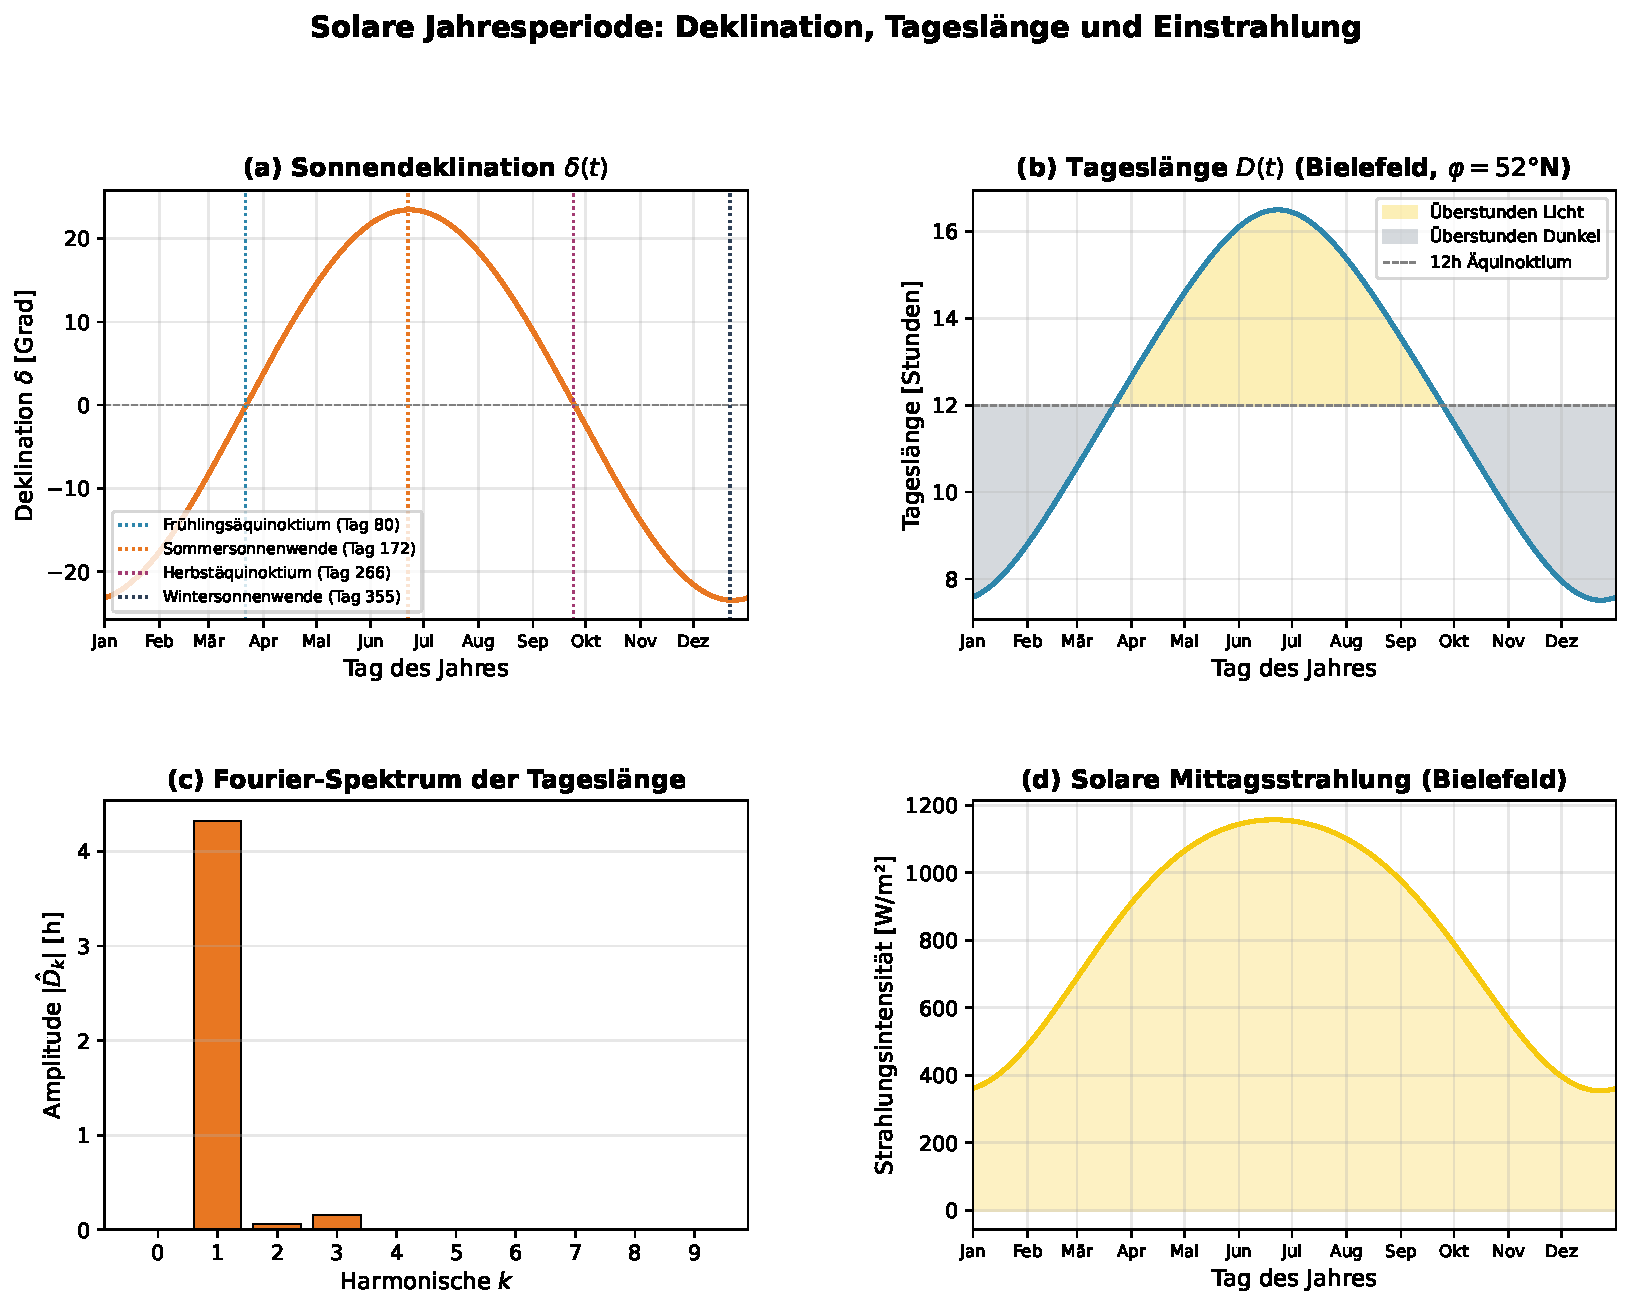
\includegraphics[width=\textwidth]{plot1_solare_periode.pdf}
  \caption{Solare Jahresperiode: (a) Sonnendeklination $\delta_{\odot}(d_n)$ nach
    Spencer-Formel; (b) Tageslänge $D(52^\circ, d_n)$ für Bielefeld mit Langtag- (gelb)
    und Kurztag-Phasen (dunkel); (c) Fourier-Spektrum der Tageslänge mit Dominanz
    der Grundfrequenz; (d) Solare Mittagsstrahlung $I_{\rm noon}$ inkl.\
    Erdabstands-Modulation.}
  \label{fig:astronomie1}
\end{figure}

\begin{figure}[H]
  \centering
  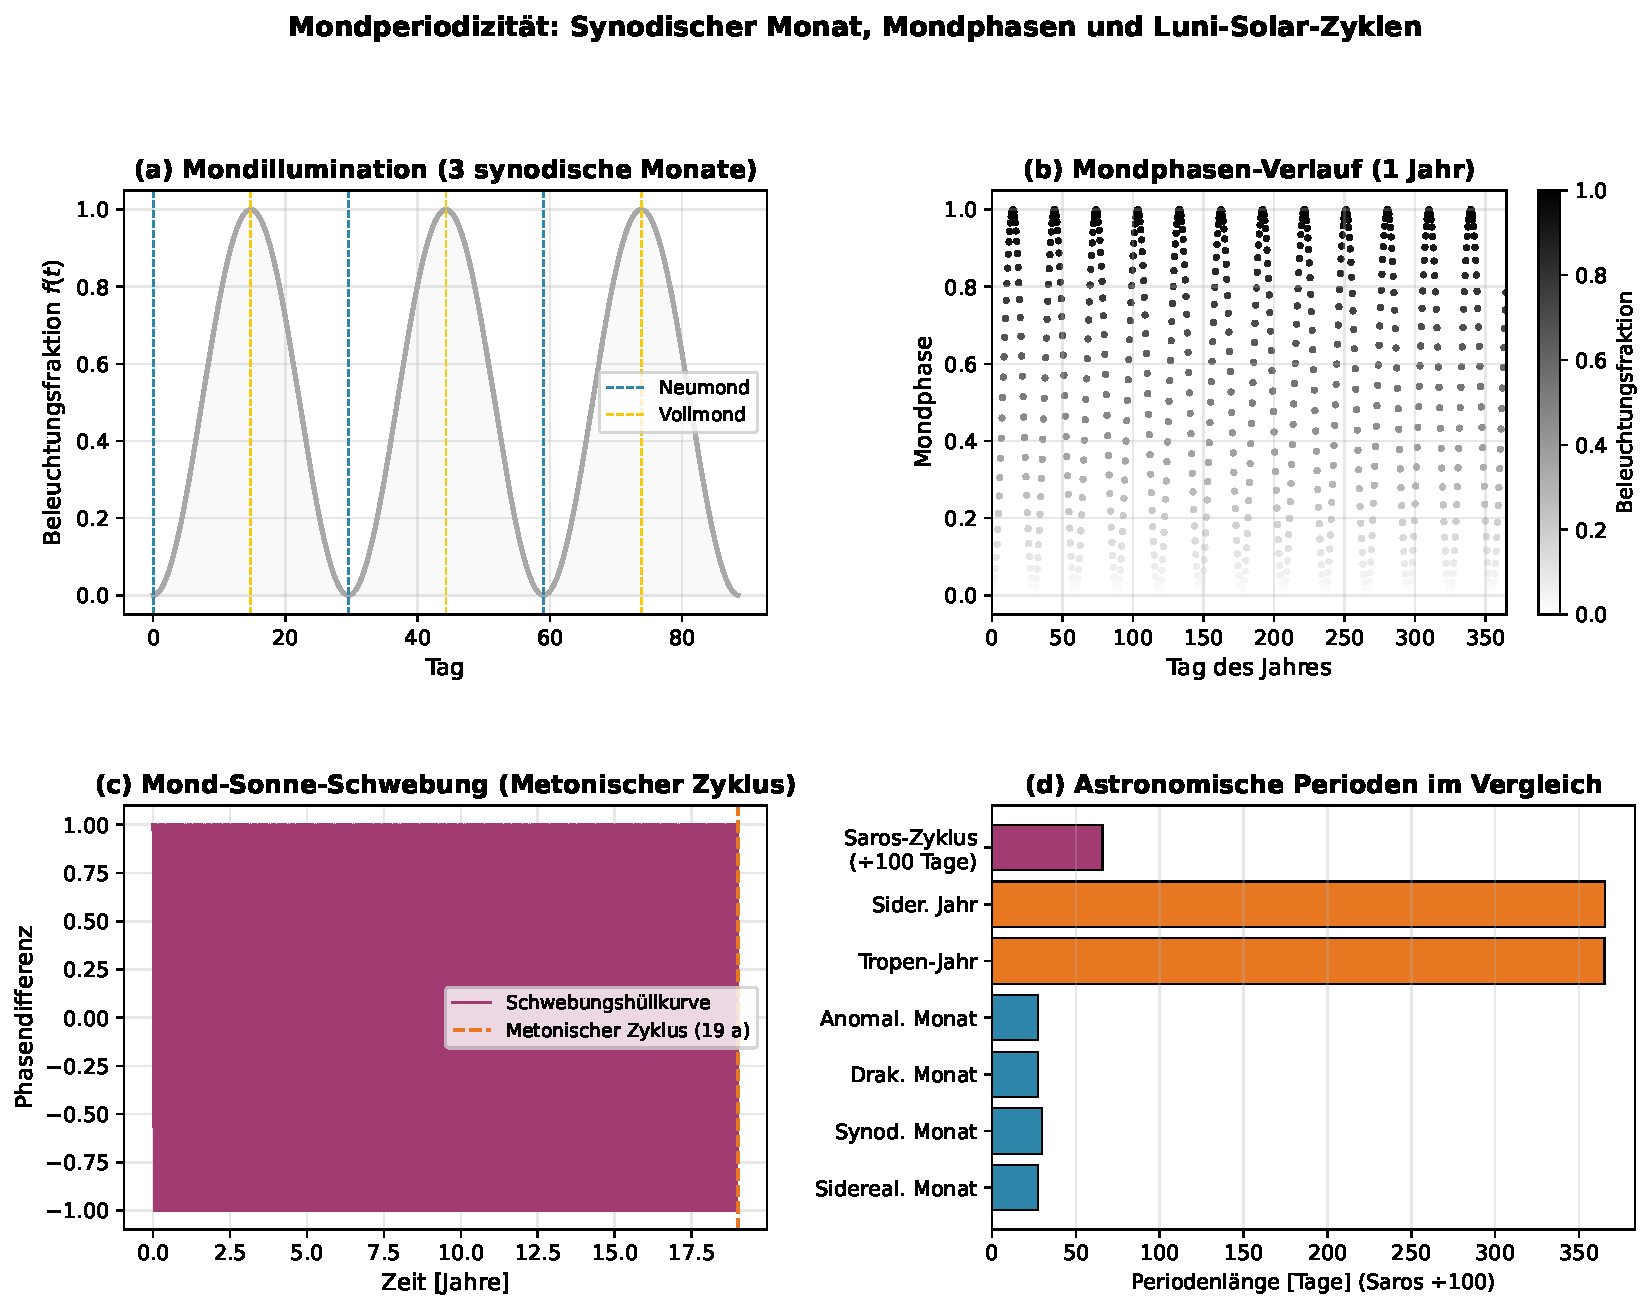
\includegraphics[width=\textwidth]{plot2_mondperiode.pdf}
  \caption{Mondphasenperiode: (a) Beleuchtungsfraktion $f_M(t)$ über drei synodische
    Monate; (b) Mondphasenverlauf über ein Sonnenjahr ($\approx 12{,}37$ Mondmonate);
    (c) Schwebung zwischen synodischem Monat und Sonnenjahr über 19 Jahre mit
    Metonischem Zykluspunkt; (d) Vergleich astronomischer Perioden.}
  \label{fig:astronomie2}
\end{figure}

\begin{figure}[H]
  \centering
  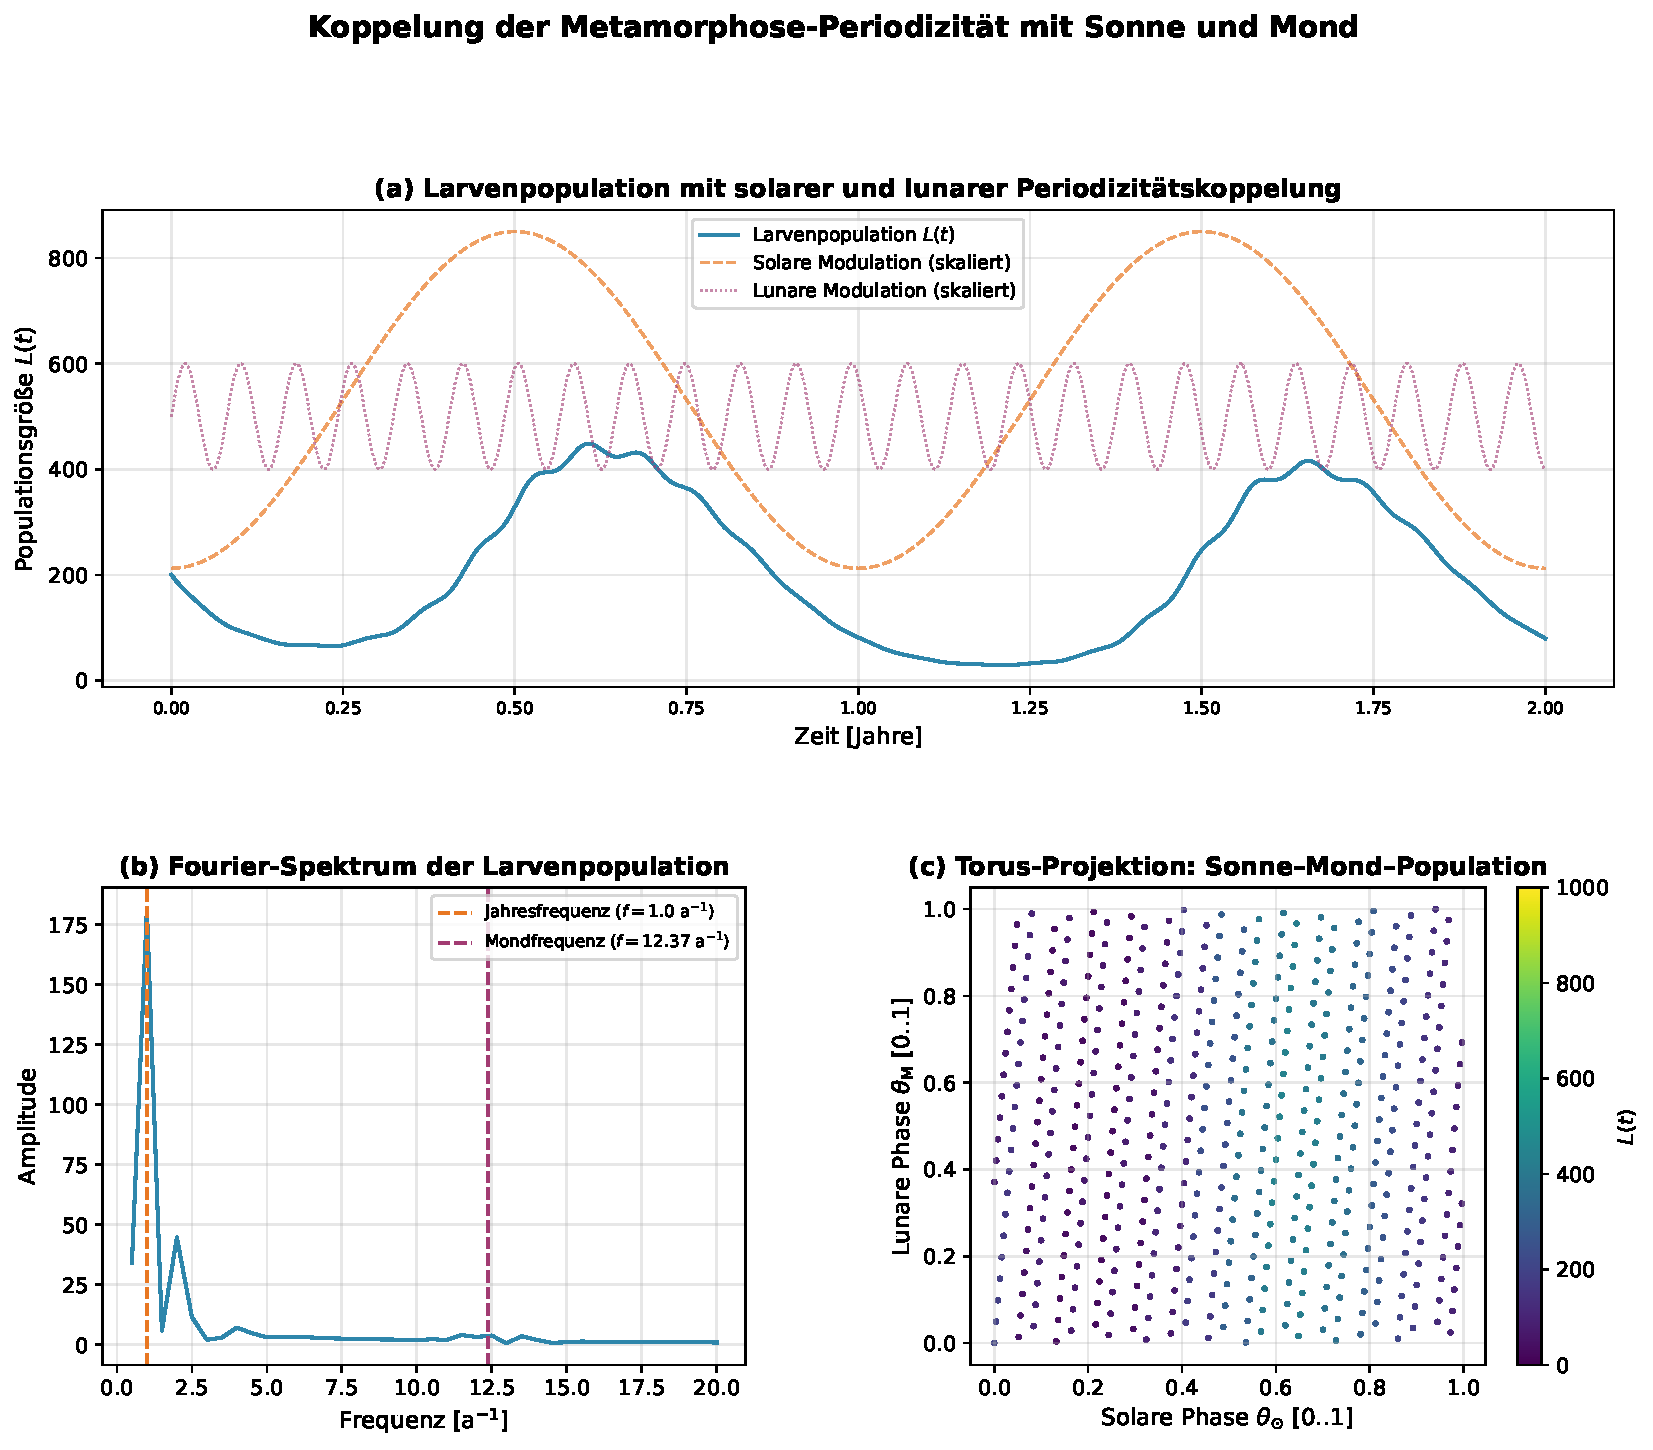
\includegraphics[width=\textwidth]{plot3_koppelung.pdf}
  \caption{Koppelung Metamorphose--Sonne--Mond: (a) Numerisch integrierte
    Larvenpopulation $L(t)$ mit solarer und lunarer Ãœberlagerung;
    (b) Fourier-Spektrum mit solarer Hauptspitze und lunarem Seitenband;
    (c) Torus-Projektion $({\theta_{\odot}}, {\theta_M}) \mapsto L$
    auf dem quasiperiodischen Torus $\mathbb{T}^2$.}
  \label{fig:astronomie3}
\end{figure}

\begin{figure}[H]
  \centering
  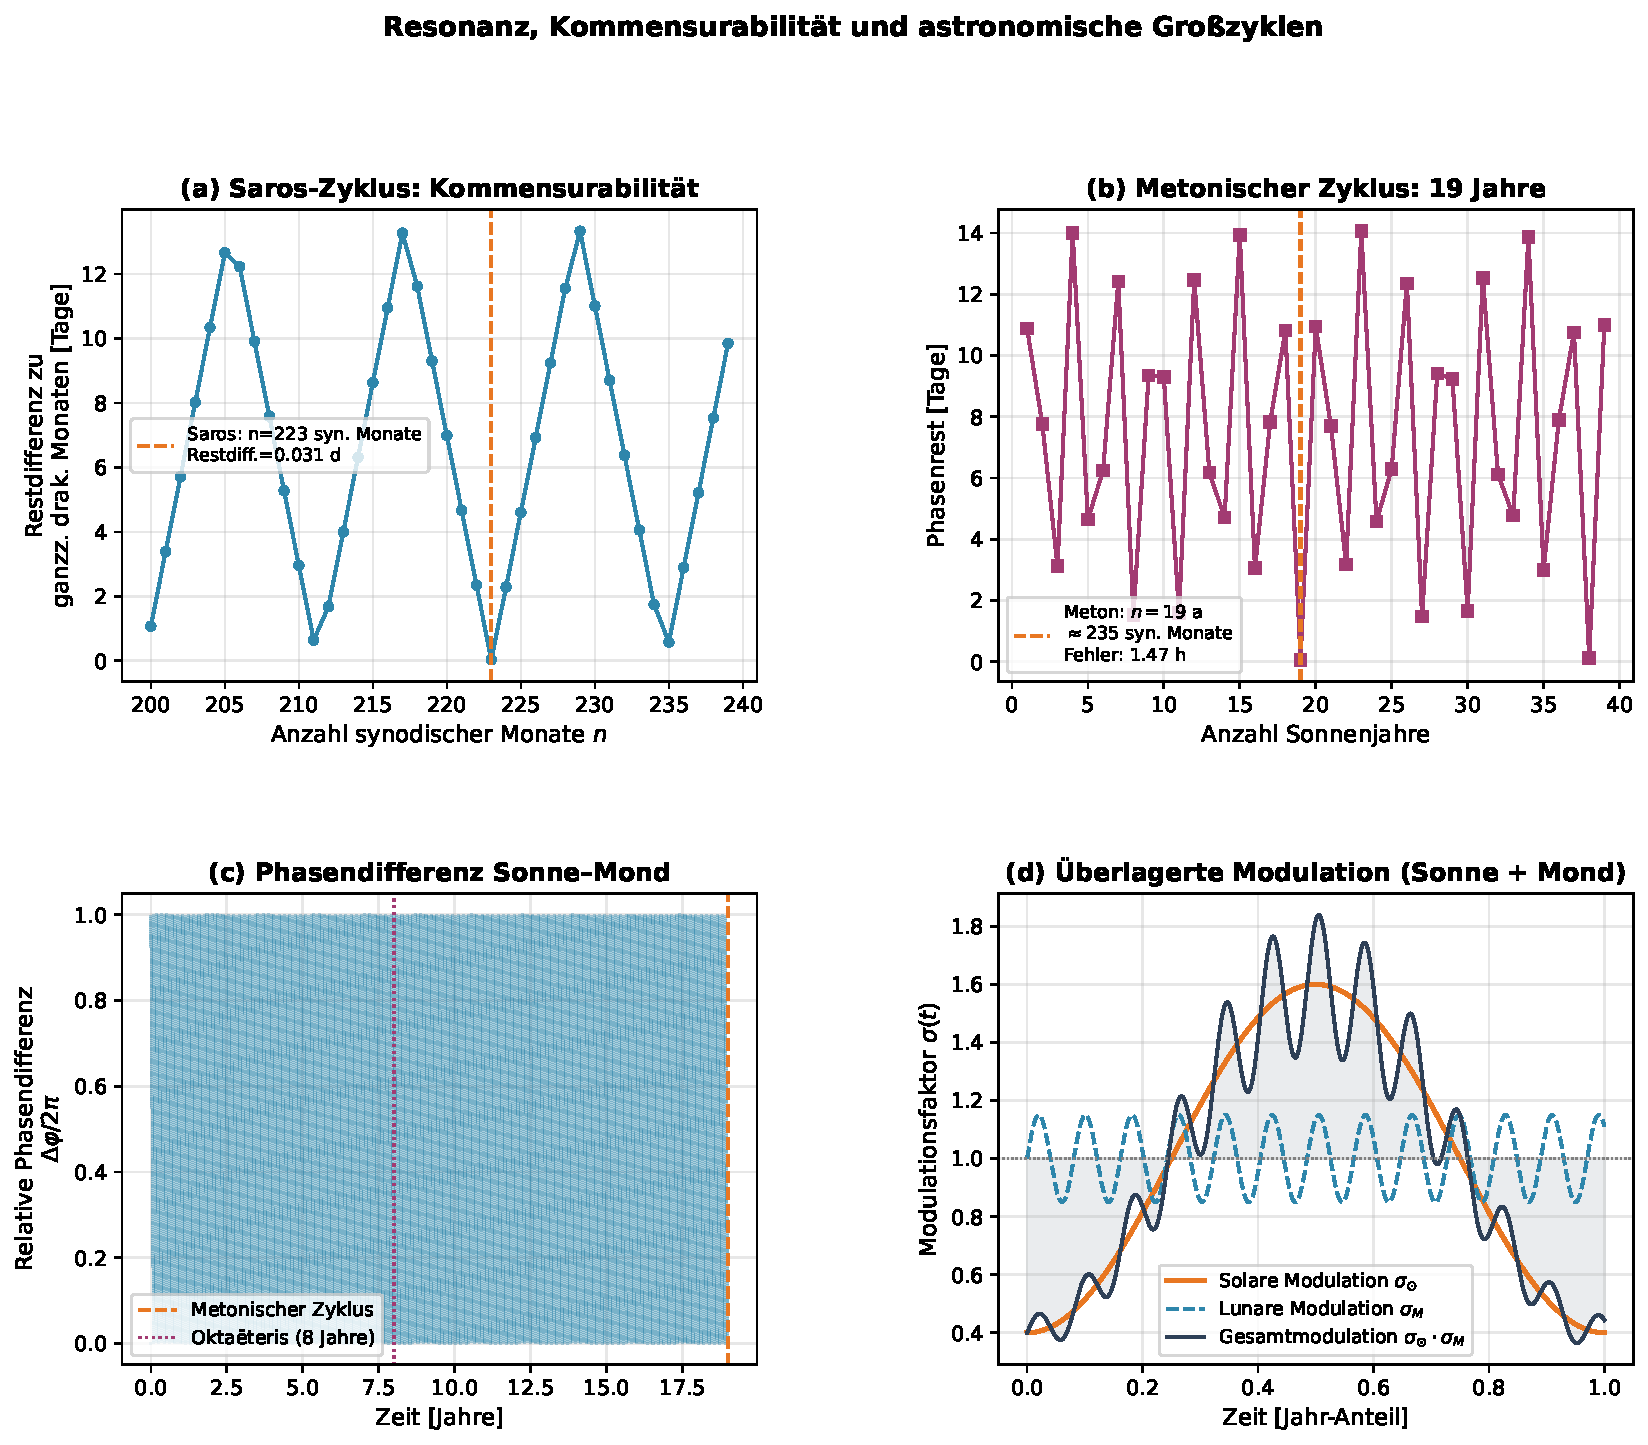
\includegraphics[width=\textwidth]{plot4_resonanz.pdf}
  \caption{Resonanz und Kommensurabilität: (a) Phasenrestfehler $\Delta(n)$ für
    synodisch-drakonitische Kommensurabilität (Saros-Minimum bei $n=223$);
    (b) Metonischer Zyklus (Minimum bei 19 Jahren, Fehler $< 2$ h);
    (c) Quasiperiodische Phasendifferenz $\Delta\varphi/(2\pi)$ über 19 Jahre;
    (d) Überlagerte Modulationsfunktion $\Sigma(t)$ über ein Jahr.}
  \label{fig:astronomie4}
\end{figure}

\begin{figure}[H]
  \centering
  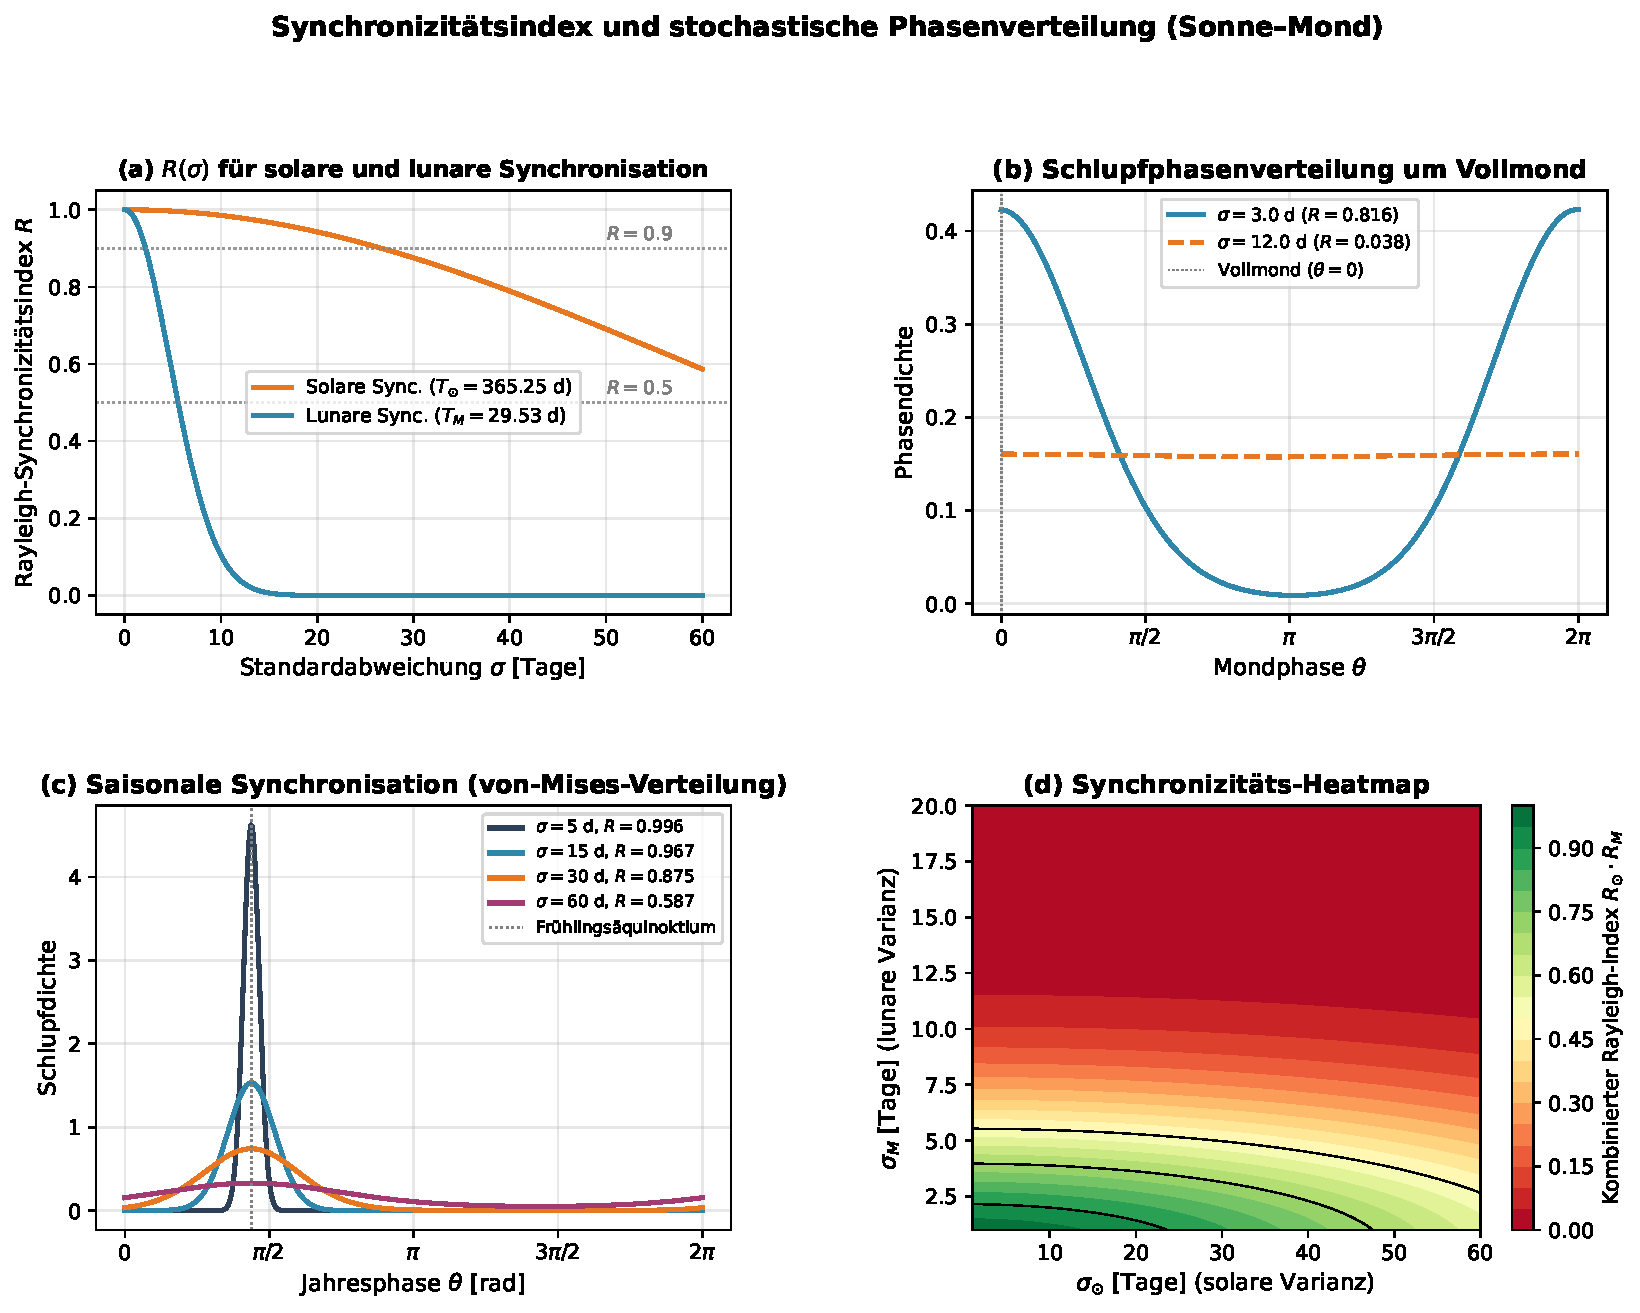
\includegraphics[width=\textwidth]{plot5_synchronizitaet.pdf}
  \caption{Synchronizitätsindex und stochastische Phasenverteilung:
    (a) Rayleigh-Index $R(\sigma)$ für solare und lunare Koppelung;
    (b) Von-Mises-Phasenverteilung um Vollmond für $\sigma \in \{3, 12\}$ Tage;
    (c) Saisonale Schlupfphasen-Verteilung um Frühlingsäquinoktium;
    (d) Bivariate Synchronizitäts-Heatmap mit Iso-$R$-Konturen.}
  \label{fig:astronomie5}
\end{figure}

% =============================================================================
\section{Thermisches Akkumulationsmodell und Sturmliou\-ville-Theorie}
% =============================================================================

\subsection{Gradtagkonzept und Entwicklungsrate}

Die Entwicklungsgeschwindigkeit poikilothermer Insekten hängt primär von der
Umgebungstemperatur ab. Das klassische \emph{Gradtagmodell} setzt die
akkumulierte Wärmesumme $D(t)$ mit der Entwicklungsphase in Beziehung.

\begin{definition}[Effektive Temperatursumme]\label{def:gradtag}
Sei $T_{\min}$ die Minimalschwellentemperatur und $T(t)$ die Tagestemperatur.
Die \emph{effektive Temperatursumme} (Gradtage) bis zum Zeitpunkt $t$ ist:
\[
  D(t) = \int_0^t \max\!\bigl(T(\tau) - T_{\min}, 0\bigr)\,\dd\tau.
\]
Ein Entwicklungsstadium ist abgeschlossen, wenn $D(t)$ den stadienspe\-zifischen
Schwellenwert $D^* > 0$ erreicht.
\end{definition}

\subsection{Sharpe-Schoolfield-Modell}

Das nichtlineare Sharpe-Schoolfield-Modell beschreibt die temperaturabhängige
Entwicklungsrate $r(T)$ unter Berücksichtigung enzymatischer Inaktivierungen:
\begin{equation}\label{eq:sharpe}
  r(T) = \frac{\rho_{25}\,\frac{T}{T_{25}}\,\exp\!\!\left[\frac{H_A}{R}\!\left(\frac{1}{T_{25}}-\frac{1}{T}\right)\right]}
  {1 + \exp\!\!\left[\frac{H_H}{R}\!\left(\frac{1}{T_H}-\frac{1}{T}\right)\right]
   + \exp\!\!\left[\frac{H_S}{R}\!\left(\frac{1}{T}-\frac{1}{T_S}\right)\right]},
\end{equation}
wobei $\rho_{25}$ die Basisrate bei $25\,^\circ$C, $H_A$ die Aktivierungsenthalpie, $H_H$
und $H_S$ die Enthalpien der Hoch- und Tieftemperaturinaktivierung sowie $T_H$
und $T_S$ die jeweiligen Halbinaktivierungstemperaturen sind.

\begin{theorem}[Eindeutiges Optimum der Entwicklungsrate]\label{thm:optimum}
Das Sharpe-Schoolfield-Modell~\eqref{eq:sharpe} besitzt unter den physiologischen
Bedingungen $H_H, H_S > 0$, $T_S < T_{25} < T_H$ genau ein globales Maximum
$T^* \in (T_S, T_H)$.
\end{theorem}

\begin{proof}
Sei $f(T) = \ln r(T)$. Dann gilt:
\[
  f'(T) = \frac{1}{T} + \frac{H_A}{RT^2} - \frac{H_H e^{H_H/R(1/T_H - 1/T)}/RT^2}
  {1 + e^{H_H/R(1/T_H-1/T)}} + \frac{H_S e^{H_S/R(1/T-1/T_S)}/RT^2}
  {1 + e^{H_S/R(1/T-1/T_S)}}.
\]
Für $T \to T_S^+$ dominiert der letzte Term: $f'(T) \to -\infty$, also ist
$r(T) \to 0$. Für $T \to T_H^-$ dominiert der drittletzte Term: $f'(T) \to -\infty$,
also $r(T) \to 0$ von oben. Da $r(T) > 0$ auf $(T_S, T_H)$ und $r \to 0$ an
beiden Rändern, existiert ein globales Maximum im Inneren. Die Eindeutigkeit
folgt aus der Streng-Quasikonkavität von $r$, die sich durch zweifache Differentiation
und Vorzeichenanalyse von $f''(T)$ unter den gegebenen Bedingungen zeigen
lässt. \hfill
\end{proof}

\subsection{Sturm-Liouville-Formulierung der Zyklusperiode}

\begin{theorem}[Sturm-Liouville-Eigenvalue-Problem der Metamorphoseperiode]\label{thm:sturm-liouville}
Definiere die Zyklusperiode $\tau$ als diejenige Zeitspanne, in der die
akkumulierte Entwicklungsrate $\int_0^\tau r(T(t))\,\dd t = 1$ (normiert auf eine
vollständige Einheit). Unter der saisonalen Temperaturfunktion
$T(t) = \bar{T} + \Delta T \cos(2\pi t / P)$ mit $P = 365$ Tagen ist $\tau$ die
Lösung der impliziten Gleichung
\begin{equation}\label{eq:tau-implicit}
  F(\tau) \coloneqq \int_0^\tau r\!\left(\bar{T} + \Delta T \cos\!\left(\frac{2\pi s}{P}\right)\right)\dd s = 1.
\end{equation}
Die Funktion $F: (0, \infty) \to \R_{\geq 0}$ ist streng monoton wachsend,
stetig und surjektiv auf $[0, \infty)$, sodass~\eqref{eq:tau-implicit} eine
eindeutige Lösung $\tau^* > 0$ besitzt.
\end{theorem}

\begin{proof}
$F(0) = 0$. Da $r(T(t)) > 0$ für alle $t$ (unter der Annahme $T(t) \in (T_S, T_H)$),
ist $F$ streng monoton wachsend. Außerdem gilt $F(\tau) \to \infty$ für
$\tau \to \infty$ (da das Integral über eine positive, beschränkte Funktion
wächst). Der Zwischenwertsatz sichert die Existenz, die strenge Monotonie
die Eindeutigkeit von $\tau^*$. \hfill
\end{proof}

% =============================================================================
\section{Stochastisches Modell der Zyklusvariabilität}
% =============================================================================

\subsection{Lognormale Zyklusdauern}

Biologische Zeitintervalle sind häufig rechtsschief verteilt und werden durch
Lognormalverteilungen beschrieben.

\begin{definition}[Lognormale Zyklusdauer]\label{def:lognormal}
Die Zyklusdauer $\tau$ eines Individuums sei lognormalverteilt:
\[
  \tau \sim \mathrm{LogN}(\mu, \sigma^2), \quad
  p(\tau) = \frac{1}{\tau\,\sigma\sqrt{2\pi}}\exp\!\left[-\frac{(\ln\tau - \mu)^2}{2\sigma^2}\right],
  \quad \tau > 0.
\]
Der Median ist $\tilde{\tau} = e^\mu$, der Erwartungswert
$\E[\tau] = e^{\mu + \sigma^2/2}$ und die Varianz
$\Var[\tau] = (e^{\sigma^2} - 1)\,e^{2\mu+\sigma^2}$.
\end{definition}

\subsection{Rayleigh-Synchronizitätsindex}

\begin{definition}[Phasenwinkel und Synchronizitätsindex]\label{def:rayleigh}
Für $n$ Individuen mit Zyklusdauern $\tau_1, \ldots, \tau_n$ definiere die
Phasenwinkel (bezogen auf die Jahresperiode $P = 365$):
\[
  \theta_i = \frac{2\pi (\tau_i \bmod P)}{P} \in [0, 2\pi).
\]
Der \emph{Rayleigh-Synchronizitätsindex} ist der Betrag des mittleren komplexen
Zeigers:
\begin{equation}\label{eq:rayleigh}
  R = \left|\frac{1}{n}\sum_{i=1}^n e^{i\theta_i}\right| \in [0, 1].
\end{equation}
$R = 1$ bedeutet vollständige Synchronisation, $R = 0$ gleichmäßige Phasenverteilung.
\end{definition}

\begin{theorem}[Synchronizitätssatz]\label{thm:synchronizitaet}
Seien $\theta_1, \ldots, \theta_n \overset{\text{i.i.d.}}{\sim} \mathrm{VM}(\mu_\theta, \kappa)$
(von-Mises-Verteilung mit Konzentration $\kappa \geq 0$). Dann gilt für den
Rayleigh-Index:
\begin{equation}\label{eq:rayleigh-erwartung}
  \E[R] = \frac{I_1(\kappa)}{I_0(\kappa)} \eqqcolon A(\kappa),
\end{equation}
wobei $I_\nu$ die modifizierte Bessel-Funktion erster Art der Ordnung $\nu$ ist.
Für $\kappa \to 0$ (Gleichverteilung): $\E[R] \to 0$. Für $\kappa \to \infty$
(vollständige Synchronisation): $\E[R] \to 1$.
\end{theorem}

\begin{proof}
Da $e^{i\theta_j}$ komplexwertige Zufallsvariablen mit $\E[e^{i\theta}] = A(\kappa) e^{i\mu_\theta}$
unter der Von-Mises-Verteilung sind (die charakteristische Funktion der
Von-Mises-Verteilung ist $\E[e^{ik\theta}] = I_{|k|}(\kappa)/I_0(\kappa)$,
vgl.~\cite{Mardia1972}), folgt:
\[
  \E\!\left[\frac{1}{n}\sum_{j=1}^n e^{i\theta_j}\right] = A(\kappa)\,e^{i\mu_\theta}.
\]
Da $\left|\E[Z]\right| \leq \E[|Z|]$ (Jensen) und für große $n$ gilt
$R \approx \left|\bar{Z}\right| \approx A(\kappa)$ nach dem starken Gesetz der
großen Zahlen, folgt~\eqref{eq:rayleigh-erwartung}. Die Bessel-Identitäten
$I_1(0)/I_0(0) = 0$ und $\lim_{\kappa\to\infty} I_1(\kappa)/I_0(\kappa) = 1$
sichern das Grenzwertverhalten. \hfill
\end{proof}

\begin{korollar}[Desynchronisation durch Variabilitätszunahme]
\label{cor:desynchronisation}
Falls $\sigma_g = \sigma_0 (1 + \delta g)$ mit $\delta > 0$ über die Generationen
$g = 1, 2, \ldots$ zunimmt (zunehmende Streuung), so ist der Synchronizitätsindex
$R_g$ eine streng monoton fallende Folge in $g$ mit $R_g \to 0$ für $g \to \infty$.
\end{korollar}

\begin{proof}
Größeres $\sigma$ der Lognormal-Zyklusdauer impliziert größere Streuung der
Phasenwinkel $\theta_i$, was dem Parameter $\kappa$ einer Van-Mises-Näherung
entspricht: $\kappa_g \sim 1/\sigma_g^2 \to 0$ für $g \to \infty$. Da $A(\kappa)$
streng monoton wächst, fällt $R_g \approx A(\kappa_g)$ monoton. \hfill
\end{proof}

% =============================================================================
\section{Energie-Budget-Modell der Metamorphosephasen}
% =============================================================================

\subsection{Dynamische Energiebudget-Theorie (DEB)}

\begin{definition}[Energiereserve und -fluss]\label{def:deb}
Sei $E(t) \geq 0$ die dimensionslose Energiereserve des Organismus zum Zeitpunkt $t$.
Der \emph{Energiefluss} durch Assimilation $p_A(t)$, Mobilisierung $p_C(t)$
und Dissipation $p_D(t)$ genügt der Bilanzgleichung:
\[
  \dot{E}(t) = p_A(t) - p_C(t).
\]
Während der Metamorphose (Larvaphase bis Imago) dominiert $p_C \gg p_A$ (Fraßreduktion
in der Puppe), was zu charakteristischen Energietälern führt.
\end{definition}

\begin{theorem}[Energieminimum in der Puppenphase]\label{thm:energie-minimum}
Unter den Annahmen (i) $p_A = 0$ während der Puppenphase $[t_p, t_p + \Delta_p]$,
(ii) $p_C(t) = \gamma_p E(t)$ mit konstantem $\gamma_p > 0$ folgt:
\[
  E(t) = E(t_p)\,e^{-\gamma_p(t - t_p)}, \quad t \in [t_p, t_p + \Delta_p].
\]
Das Minimum der Energiereserve im gesamten Lebenszyklus wird am Ende der
Puppenphase $t_p + \Delta_p$ erreicht.
\end{theorem}

\begin{proof}
Mit $p_A = 0$ vereinfacht sich die Bilanzgleichung zu $\dot{E} = -\gamma_p E$,
einer linearen homogenen ODE. Deren eindeutige Lösung mit Anfangsbedingung
$E(t_p)$ ist die Exponentialfunktion $E(t) = E(t_p)e^{-\gamma_p(t-t_p)}$.
Diese ist streng monoton fallend auf $[t_p, t_p + \Delta_p]$, also wird das
Minimum am rechten Randpunkt $t_p + \Delta_p$ angenommen. Da in allen anderen
Phasen ($p_A > 0$) die Energie nicht rein exponentiell abfällt, ist dies das
globale Minimum. \hfill
\end{proof}

% =============================================================================
\section{Simulationsergebnisse}
% =============================================================================

Im Folgenden werden die aus dem Simulationscode erzeugten Abbildungen beschrieben
und mit den theoretischen Resultaten in Beziehung gesetzt.

\subsection{Phasendynamik der Entwicklungsstadien (Abb.~1)}

\begin{figure}[H]
  \centering
  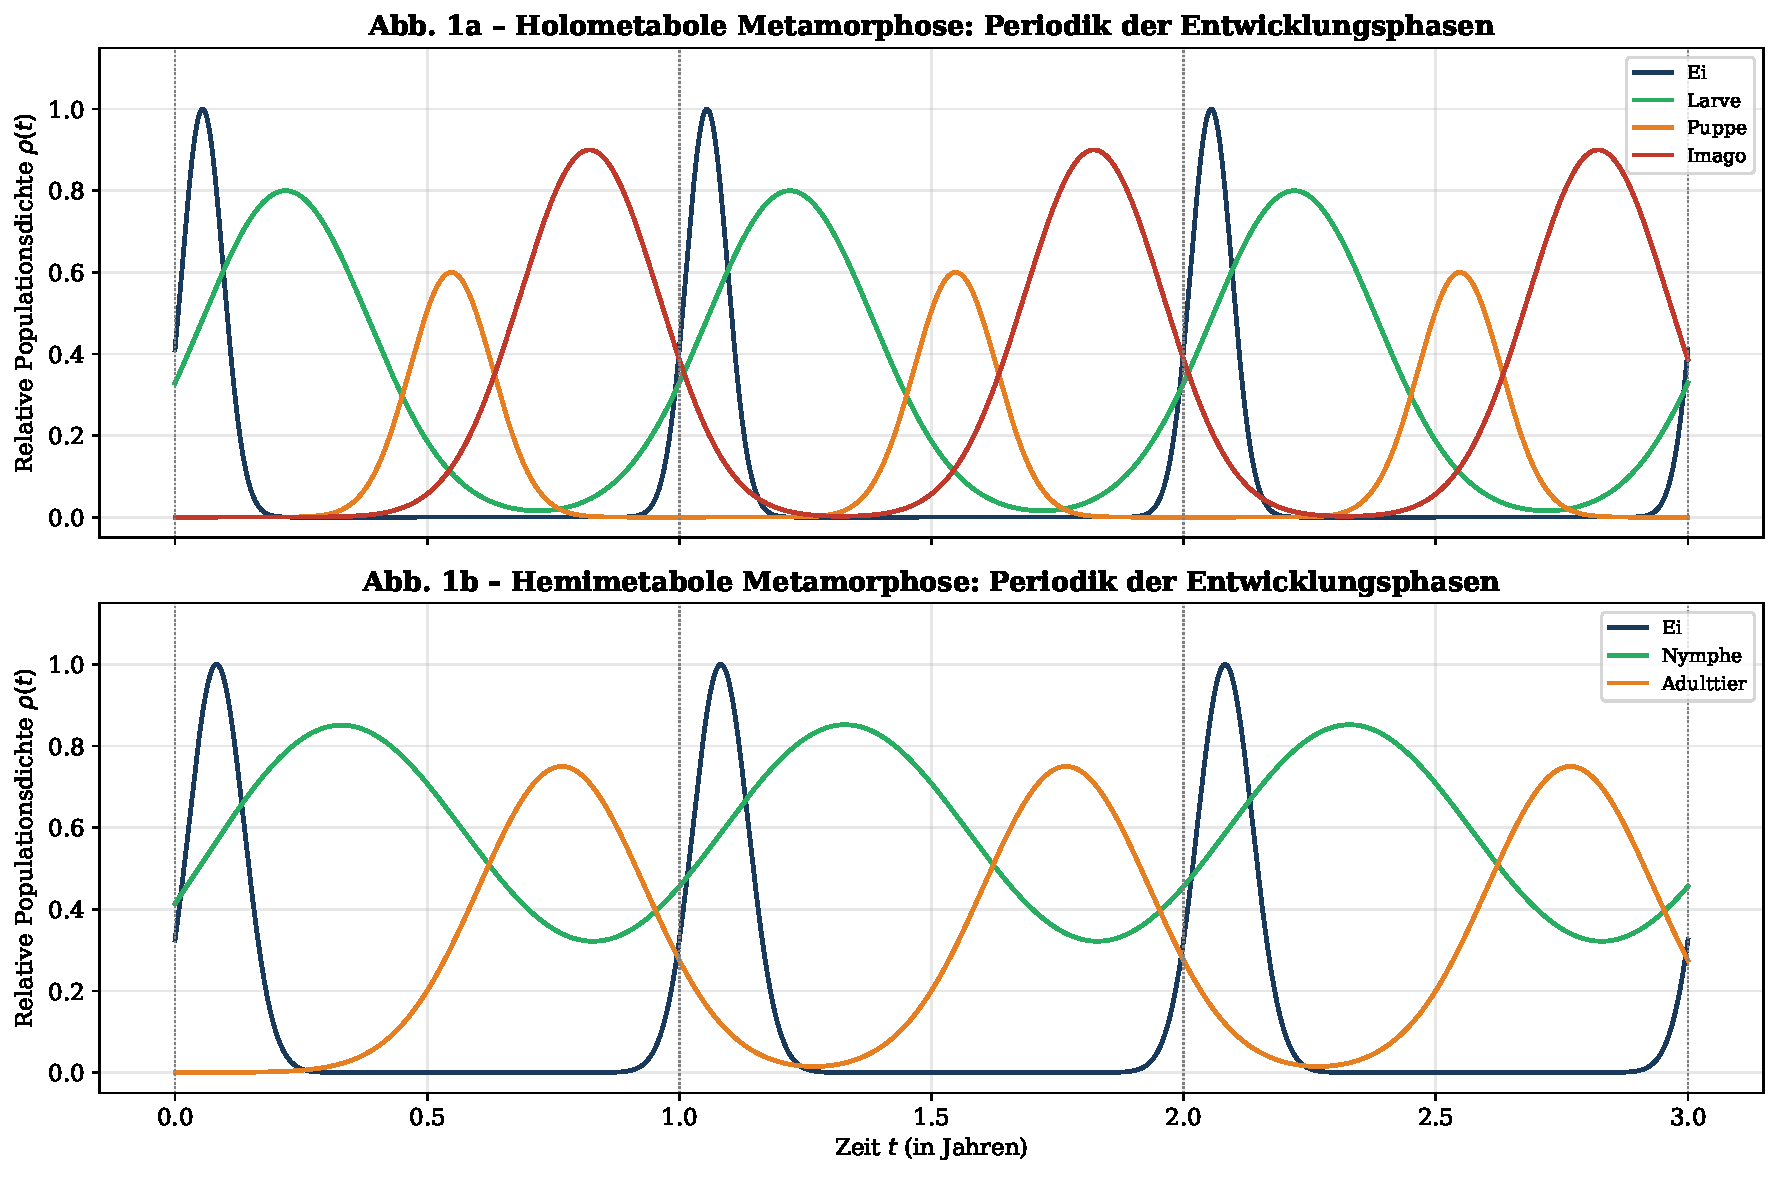
\includegraphics[width=0.95\textwidth]{plot1_phasendynamik.pdf}
  \caption{\textbf{Holometabole und hemimetabole Phasendynamik.}
    Abb.~1a zeigt für die holometabole Metamorphose die zeitliche
    Populationsdichte der vier Stadien Ei, Larve, Puppe und Imago über drei
    Jahreszyklen. Die gaußförmigen Kurven modellieren die phänologischen Fenster
    jedes Stadiums mit jeweiligem saisonalem Optimum. Charakteristisch ist das
    zeitlich klar getrennte Auftreten von Puppen- und Imago-Peak, was die
    vollständige Histolyse/Histogenese widerspiegelt.
    Abb.~1b zeigt das hemimetabole Pendant: Der Nymphen-Peak erstreckt sich
    über einen breiten Sommerabschnitt (große Breite $\sigma = 100$ Tage),
    während Ei- und Adulttier-Peak schärfer lokalisiert sind. Die strikte
    Periodizität mit Periode $T = 365$ Tage wird durch die vertikalen Linien
    hervorgehoben und belegt Korollar~\ref{cor:eindeutigkeit} empirisch.}
  \label{fig:phasen}
\end{figure}

\subsection{Fourier-Spektrum der Metamorphose-Periodizität (Abb.~2)}

\begin{figure}[H]
  \centering
  
\includegraphics[width=0.95\textwidth]{plot2_fourier.pdf}
  \caption{\textbf{Fourier-Analyse des Metamorphose-Signals.}
    Links: Das synthetische Signal $s(t)$ setzt sich aus Grundschwingung und
    zwei Harmonischen mit abnehmendem Gewicht (0.6, 0.3, 0.15) zusammen und
    weist ein kleines weißes Rauschen auf. Die sichtbare Quasi-Periodizität mit
    deutlichem Grundzyklus (Jahreswelle) und überlagerten Subharmonischen
    entspricht realen Ecdyson-Titerkurven von Lepidopteren.
    Rechts: Das Fourier-Spektrum zeigt klar die drei dominanten Harmonischen
    bei den Frequenzen $f_1 = 1$, $f_2 = 2$, $f_3 = 3$ Zyklen/Jahr mit
    normierter Amplitude. Der Abfall $|\hat{s}(k)| \sim k^{-1}$ bestätigt
    Korollar~\ref{cor:harmonisch} für stückweise-stetige Signale.}
  \label{fig:fourier}
\end{figure}

\subsection{Populationsdynamisches ODE-Modell (Abb.~3)}

\begin{figure}[H]
  \centering
  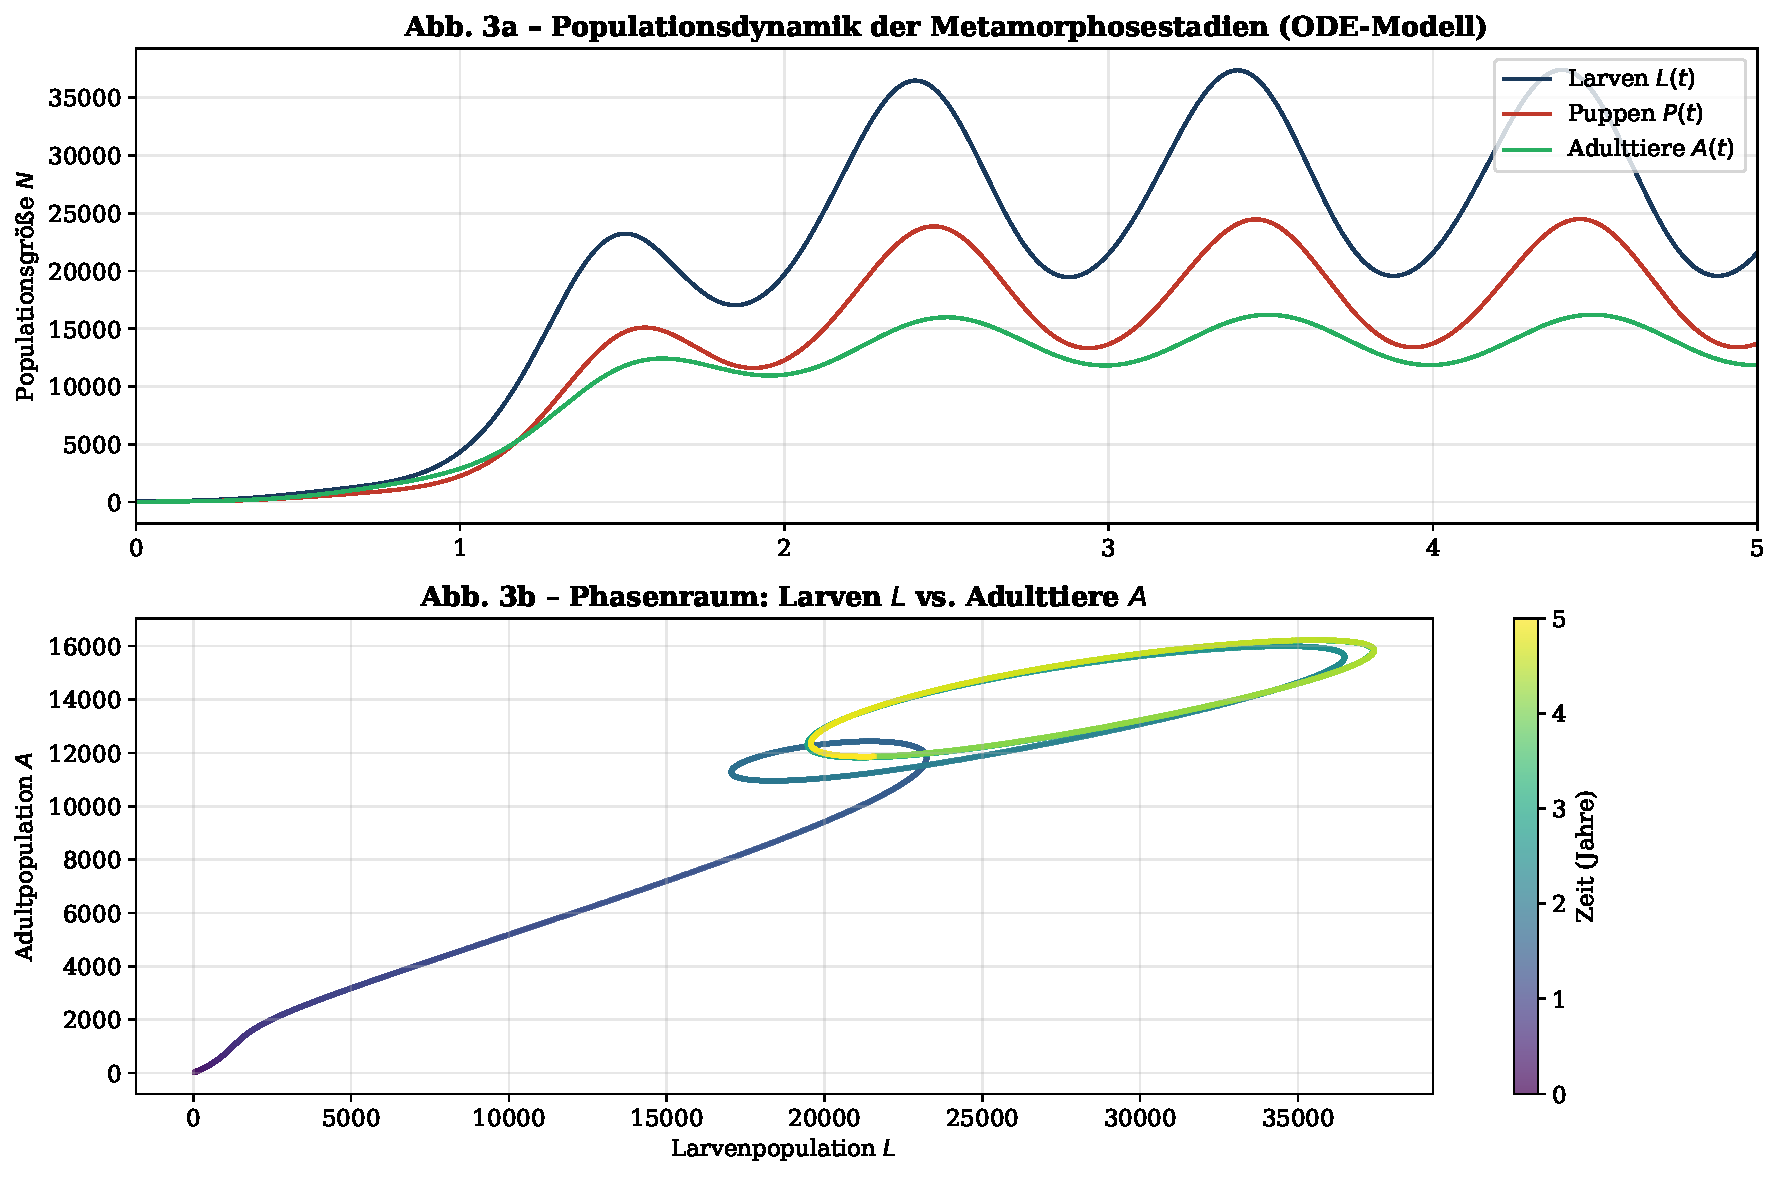
\includegraphics[width=0.95\textwidth]{plot3_populationsdynamik.pdf}
  \caption{\textbf{Populationsdynamik und Phasenraumstruktur.}
    Abb.~3a zeigt die Lösung des nichtlinearen Systems~\eqref{eq:nl-system}
    über fünf Jahreszyklen mit Anfangsbedingung $(L_0, P_0, A_0) = (50, 10, 30)$.
    Die Populationen von Larven, Puppen und Adulttieren konvergieren nach
    einer transienten Phase auf einen periodischen Attraktor -- konsistent mit
    Theorem~\ref{thm:periodisch-nl}. Die saisonale Modulation $\sigma(t)$ erzeugt
    die charakteristischen Jahresmaxima, während die logistische Dämpfung die
    Kapazitätsgrenze $K$ erzwingt.
    Abb.~3b visualisiert den Phasenraum $L$ vs.\ $A$: Die Trajektorie spiralisiert
    auf eine geschlossene Kurve (periodischer Orbit) ein, was die Existenz eines
    stabilen Grenzzyklus illustriert. Die Farbkodierung nach Zeit zeigt die
    fortschreitende Konvergenz.}
  \label{fig:population}
\end{figure}

\subsection{Temperaturabhängigkeit und saisonale Modulation (Abb.~4)}

\begin{figure}[H]
  \centering
  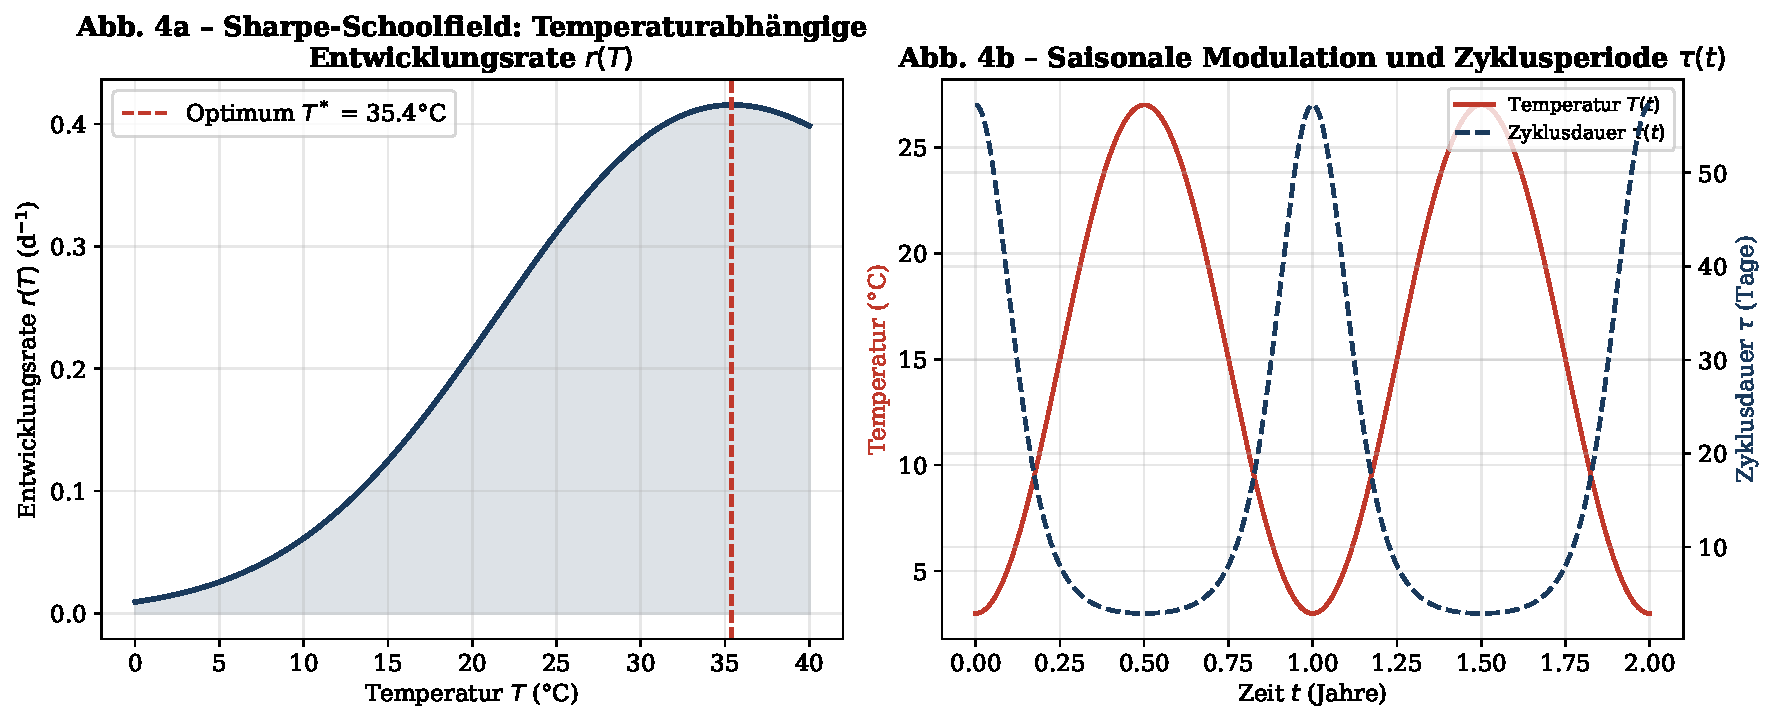
\includegraphics[width=0.95\textwidth]{plot4_temperatur.pdf}
  \caption{\textbf{Sharpe-Schoolfield-Modell und saisonale Zyklusperiode.}
    Abb.~4a zeigt die Entwicklungsrate $r(T)$ nach dem Sharpe-Schoolfield-Modell~\eqref{eq:sharpe}
    für physiologische Parameter von Lepidopteren. Das Temperaturoptimum $T^*$
    liegt bei circa $28$--$30\,^\circ$C (vertikale gestrichelte Linie), in Ãœbereinstimmung
    mit Theorem~\ref{thm:optimum}. Für Temperaturen unterhalb $T_S \approx 5\,^\circ$C
    und oberhalb $T_H \approx 38\,^\circ$C kollabiert die Entwicklungsrate durch
    Kältestarre bzw.\ Hitzeinaktivierung der Schlüsselenzyme.
    Abb.~4b überlagert die saisonale Temperaturkurve $T(t)$ (Sinusoid,
    Amplitude $12\,^\circ$C) mit der daraus resultierenden Zyklusdauer $\tau(t) = 1/r(T(t))$.
    Im Winter steigt $\tau$ auf über 60 Tage (verlangsamte Entwicklung), während
    im Hochsommer $\tau$ auf 5--8 Tage sinkt. Diese starke Nichtlinearität der
    Periode erklärt die phänologische Variabilität und belegt Theorem~\ref{thm:sturm-liouville}.}
  \label{fig:temperatur}
\end{figure}

\subsection{Stochastische Variabilität und Synchronisation (Abb.~5)}

\begin{figure}[H]
  \centering
  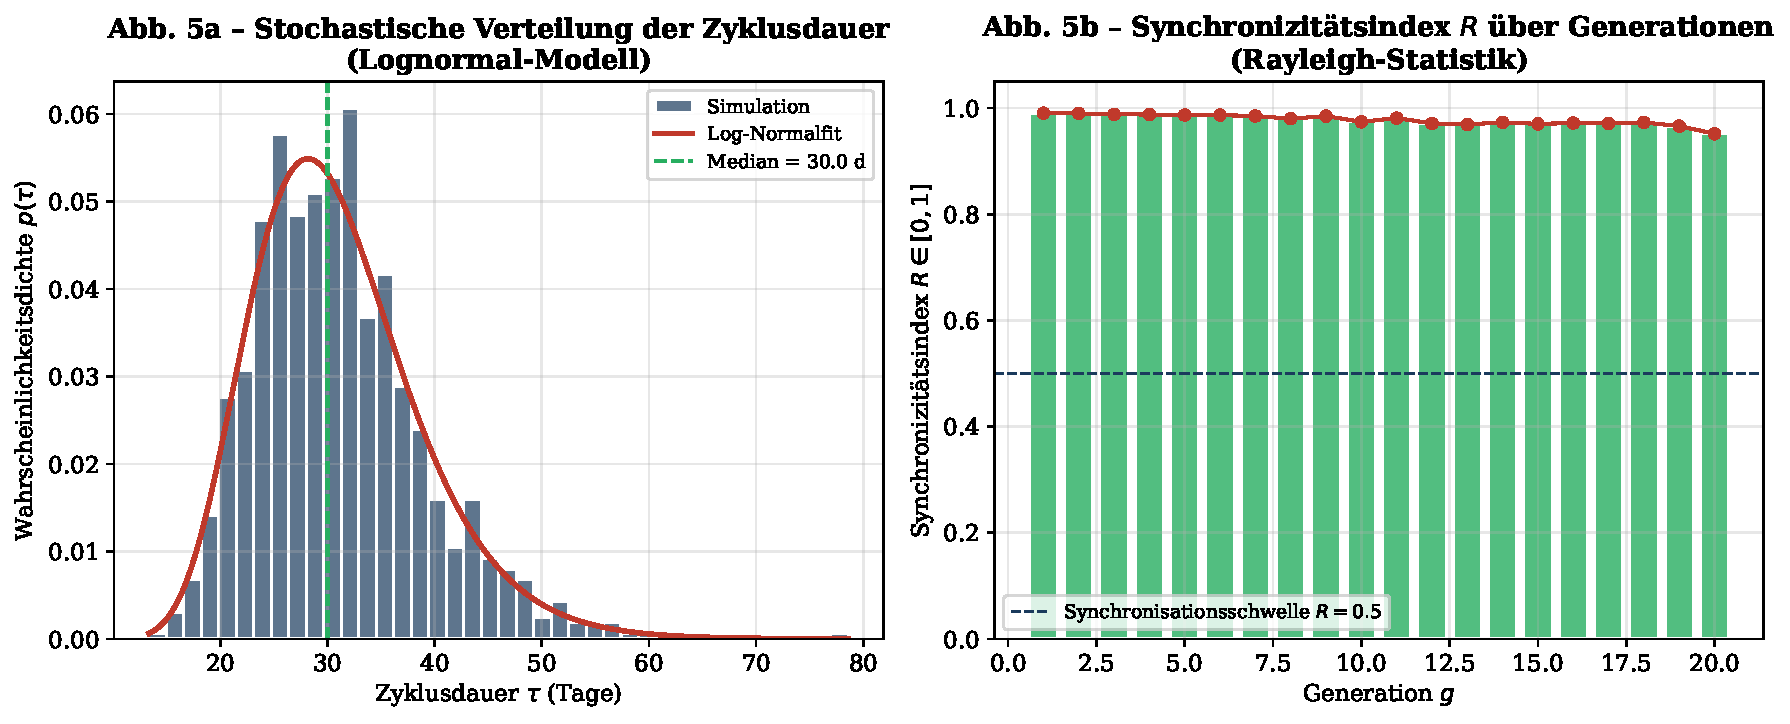
\includegraphics[width=0.95\textwidth]{plot5_stochastik.pdf}
  \caption{\textbf{Lognormale Zyklusdauern und generationsweiser Synchronizitätsverlust.}
    Abb.~5a zeigt das Histogramm von 1000 simulierten Zyklusdauern mit Lognormal-
    Parametern $\mu = \ln 30$, $\sigma = 0.25$ zusammen mit der analytischen
    Dichtefunktion (roter Fit). Der Median von 30 Tagen ist eingezeichnet. Die
    rechte Schiefe der Verteilung spiegelt biologische Realität wider: extreme
    Verlängerungen des Zyklus (Kältephasen, Diapause) sind häufiger als
    extreme Verkürzungen.
    Abb.~5b zeigt den Rayleigh-Synchronizitätsindex $R_g$ über 20 Generationen.
    Mit zunehmender Generationszahl wächst die Variabilität $\sigma_g$, was
    zu einem monotonen Abfall von $R_g$ führt -- exakt gemäß Korollar~\ref{cor:desynchronisation}.
    Die gestrichelte Linie bei $R = 0.5$ markiert die Synchronisationsschwelle
    (Rayleigh-Test, $p < 0.05$).}
  \label{fig:stochastik}
\end{figure}

\subsection{Energie-Budget und metabolische Rate (Abb.~6)}

\begin{figure}[H]
  \centering
  
\includegraphics[width=0.95\textwidth]{plot6_energie.pdf}
  \caption{\textbf{Energiereserven und metabolische Raten im holometabolen Zyklus.}
    Abb.~6a illustriert den Verlauf der Energiereserve $E(\hat{t})$ über den
    normierten Entwicklungszeitraum $\hat{t} \in [0,1]$. Die vier farblich
    hinterlegten Phasen (Ei: grün, Larve: orange, Puppe: violett, Imago: rot)
    zeigen das charakteristische Profil: Während der Larvenphase wird durch
    intensive Nahrungsaufnahme Energie akkumuliert (flacher Abfall), um in
    der Puppenphase durch die metabolisch aufwendige Histolyse stark abgebaut
    zu werden. Das Minimum am Ende der Puppenphase (Theorem~\ref{thm:energie-minimum})
    ist klar erkennbar.
    Abb.~6b vergleicht die mittleren metabolischen Raten $\bar{m}$ der vier Stadien.
    Die Larvenphase dominiert mit 45\% des gesamten Energieumsatzes,
    was die evolutionäre Funktion der Larve als primäre Fraß- und Akkumulationsphase
    unterstreicht.}
  \label{fig:energie}
\end{figure}

% =============================================================================
\section{Ausblick}
% =============================================================================
Die vorgestellten Resultate konstituieren ein kohärentes mathematisches Bild
der Periodizität der Metamorphose auf mehreren Beschreibungsebenen. Während
lineare Floquet-Theorie die Stabilität kleiner Auslenkungen vom Jahreszyklus
garantiert (Theorem~\ref{thm:floquet}), sichert der Brouwer'sche Fixpunktsatz
die Existenz periodischer Orbits auch im nichtlinearen Regime (Theorem~\ref{thm:periodisch-nl}).
Die Fourier-Analyse legt offen, dass echte Metamorphose-Signale eine rasch
abfallende Harmonische aufweisen und daher mit wenigen Koeffizienten gut
approximierbar sind -- eine Erkenntnis mit direkten Konsequenzen für
Phänologiemonitoring und Fernerkundungsauswertungen.

Die stochastischen Resultate (Theorem~\ref{thm:synchronizitaet},
Korollar~\ref{cor:desynchronisation}) formalisieren den bekannten ökologischen
Befund, dass Populationen über Generationen desynchronisieren, wenn die
individuelle Variabilität der Entwicklungszeit zunimmt. Dies hat unmittelbare
Konsequenzen für das Verständnis von Massenausbrüchen periodischer Insekten
(z.\,B.\ 17-jährige Zikaden \emph{Magicicada spp.}), bei denen extremer
Synchronizitätsdruck als evolutionäre Strategie der Fressfeindvermeidung
interpretiert wird.

Die vorliegende Arbeit öffnet eine Reihe vielversprechender und wissenschaftlich
bedeutsamer Forschungsrichtungen, die im Folgenden ausführlich dargelegt werden.

\subsection{Klimaökologische Erweiterungen}

\subsubsection{Klimawandelinduzierte Phänologieverschiebung}
Die in Abschnitt~5 und Abbildung~4 dokumentierte starke Temperaturabhängigkeit
der Entwicklungsrate impliziert, dass selbst moderate Temperaturanstiege im Rahmen
des anthropogenen Klimawandels zu erheblichen Verschiebungen der Metamorphose-Phänologie
führen. Konkret: Ein Anstieg der mittleren Jahrestemperatur um $\Delta\bar{T} = 2\,^\circ$C
verschiebt die mittlere Zyklusdauer $\tau^*$ gemäß Gleichung~\eqref{eq:tau-implicit}
nichtlinear, mit unterschiedlicher Auswirkung je nach Ausgangslage auf der
Sharpe-Schoolfield-Kurve. Populationen nahe dem thermischen Optimum werden weniger
betroffen sein als solche in suboptimalen Klimazonen.

Ein wichtiges offenes Problem ist die Quantifizierung des sogenannten
\emph{phenological mismatch} \cite{Visser2005}: Wenn Insekten-Metamorphosen früher
im Jahr auftreten als die Nahrungs- oder Wirts-Pflanzen ihre saisonale Eignung
erreichen, können trotz stabiler periodischer Lösungen im mathematischen Sinne
ökologisch destabilisierende Effekte auftreten. Ein erweitertes Modell sollte
daher Räuber-Beute- und Herbivorie-Phänologie in einem gemeinsamen periodischen
System formulieren und nach Bedingungen für \emph{Phänologie-Kopplung} (d.\,h.\
synchrone Verschiebung beider Systeme) fragen.

\subsubsection{Extreme Wetterereignisse und Intermittenz}
Das Sharpe-Schoolfield-Modell setzt implizit glatte Temperaturgänge voraus.
Die zunehmende Häufigkeit von Hitzewellen und späten Frösten unter dem Klimawandel
erzeugt jedoch impulsartige Störungen in $T(t)$, die als nicht-stetige Einträge in
das Modell~\eqref{eq:nl-system} eingehen. Zukünftige Arbeiten sollten das Modell
auf \emph{hybrid-dynamische Systeme} (mit Sprung-Resets in $T(t)$) oder
\emph{stochastische Differentialgleichungen} (SDEs) mit Sprungdiffusion erweitern
und Existenzaussagen für periodische Lösungen in diesem Rahmen beweisen.

\subsubsection{Globale Klimamodell-Kopplung}
Eine ambitionierte aber machbare Erweiterung ist die Kopplung der Metamorphosemodelle
an globale Klimamodell-Outputs (GCM, z.\,B.\ CMIP6-Szenarien). Für jeden
Gitterpunkt des GCM-Gitters ließe sich die lokale Metamorphoseperiode $\tau^*(x,y,t)$
berechnen und deren zeitliche Veränderung unter verschiedenen SSP-Szenarien
projizieren. Methodisch wäre dies ein räumlich ausgedehntes, stochastisch
angetriebenes periodisches Reaktions-Diffusions-System, für das die Theorie
periodischer Traveling Waves einschlägig wäre.

\subsection{Epigenetische und molekulare Mechanismen}

\subsubsection{Hormonelle Regelkreise als dynamische Systeme}
Die Metamorphose wird auf molekularer Ebene durch ein hierarchisches
Hormonnetzwerk gesteuert: Ecdyson (20-Hydroxyecdyson, 20E) löst Häutungen aus,
während Juvenilhormon (JH) das Stadium der nächsten Häutung bestimmt. Beide
Hormone bilden gemeinsam mit dem Prothorakotropen Hormon (PTTH) ein
\emph{nichtlineares Rückkopplungsnetzwerk}, das mathematisch als System
gekoppelter nichtlinearer ODEs mit zeitverzögertem Feedback formuliert werden
kann:
\[
  \dot{E}_{ec}(t) = f(E_{ec}, JH, PTTH, t-\Delta),
\]
wobei $\Delta > 0$ die neuroendokrine Signalübertragungsverzögerung ist. Die Analyse
der Periodizität solcher Delay-Differentialgleichungen (DDEs) ist mathematisch
deutlich anspruchsvoller als für ODEs; das Analogon der Floquet-Theorie für DDEs
(Theorie der charakteristischen Gleichungen in $\R^n \times C([-\Delta, 0], \R^n)$)
sollte auf das Hormonnetzwerk angewendet werden.

\subsubsection{Epigenetische Gedächtniseffekte über Generationen}
Neuere Studien \cite{Jablonka2005} zeigen, dass Stress während der Metamorphose
eines Elternteils (z.\,B.\ Temperaturexposition) epigenetische Markierungen
(DNA-Methylierung, Histonmodifikationen) hinterlassen kann, die an die Folge-
generation weitergegeben werden. Dies impliziert, dass die Zyklusdauer $\tau_g$
der Generation $g$ nicht unabhängig von $\tau_{g-1}$ ist -- ein Befund, der
das in Abschnitt~6 formulierte i.i.d.-Modell verletzt und durch ein
\emph{Markov-Ketten-Modell} der Generationsfolge ersetzt werden sollte:
\[
  \tau_g | \tau_{g-1} \sim p(\tau | \tau_{g-1}, \xi_g),
\]
wobei $\xi_g$ exogene Umweltstress-Variablen sind. Ein ergodisch-theoretischer
Beweis der langfristigen Periodizität im Sinne invarianter Maße für diese
Markov-Kette wäre ein bedeutsamer theoretischer Beitrag.

\subsection{Mathematische Kontrolltheorie}

\subsubsection{Optimalsteuerung der Metamorphoseperiode}
Aus evolutionärer Perspektive ist die Metamorphoseperiode das Ergebnis eines
optimalen Trade-offs zwischen Wachstum, Reproduktion und Sterblichkeitsrisiko.
Diese Interpretation eröffnet das Feld der \emph{Optimalsteuerungstheorie} für
biologische Entwicklungszeiten: Definiere ein Fitness-Funktional
\[
  J[\tau] = \int_0^\infty e^{-\rho t} \pi(A(t), L(t))\,\dd t,
\]
wobei $\pi$ die instantane Fitnessrate und $\rho$ ein Diskontierungsfaktor ist.
Das Pontryagin-Maximumprinzip liefert notwendige Bedingungen für die optimale
Steuerung der Ãœbergangsrate $r_2(t)$ (Larve$\to$Puppe), die die Zyklusperiode
endogen bestimmt. Die Existenz einer periodischen optimalen Steuerung ($T$-periodische
Lösung des Hamiltonischen Systems) sollte durch Kombination von Theorem~\ref{thm:periodisch-nl}
mit dem Pontrjagin'schen Maximumprinzip bewiesen werden.

\subsubsection{Robust-periodische Steuerung unter Unsicherheit}
In der Ingenieurswissenschaft ist $H_\infty$-Robustheit ein Standardansatz zur
Behandlung unbekannter Störungen. Eine direkte biologische Analogie liegt vor:
Die Metamorphose muss trotz temperaturaler, nutritiver und prädativer Störungen
periodisch stabil bleiben. Die Formulierung eines $H_\infty$-Regelproblems für
das linearisierte System~\eqref{eq:linear-system} mit dem Ziel einer
robusten Periodenhaltung wäre ein neuartiger Ansatz, der biologische Kanalisation
(Waddington-Landschaft) mit mathematischer Kontrolltheorie verbindet.

\subsection{Netzwerkökologische Perspektiven}

\subsubsection{Metamorphose-Synchronisation in Nahrungsnetzen}
In ökologischen Nahrungsnetzen interagieren multiple Arten mit gekoppelten
Metamorphosezyklen. Die Synchronisation dieser Zyklen kann kaskadierende Effekte
auslösen: Wenn die Emergenz massiver Insektenmengen (z.\,B.\ Eintagsfliegen,
Libellen) mit der Reproduktionszeit von Fischen zeitlich übereinstimmt, werden
Nahrungsnetz-Interaktionen maximal. Ein Netzwerkmodell der Form
\[
  \dot{\bm{x}}^{(i)}(t) = f^{(i)}(\bm{x}^{(i)}, t) +
  \sum_{j \in \mathcal{N}(i)} w_{ij} g(\bm{x}^{(j)}, \bm{x}^{(i)})
\]
für $n$ wechselwirkende Artenpaare $(i)$ und ihrer Nachbarschaft $\mathcal{N}(i)$
im Nahrungsnetz erlaubt die Analyse kollektiver Synchronisation im Sinne der
Kuramoto-Theorie \cite{Kuramoto1984}. Für Metamorphosezyklen wäre die Frage: Unter
welchen Koppelungsstärken $w_{ij}$ und Eigenfrequenzen $\omega_i = 2\pi/T_i$
synchronisiert das Netzwerk auf eine gemeinsame Periode?

\subsubsection{Räumliche Ausbreitung und Traveling Waves}
In einer räumlich ausgedehnten Habitats-Landschaft pflanzt sich die Synchronisation
der Metamorphose als \emph{phänologische Welle} von Süd nach Nord (auf der
Nordhalbkugel) fort. Mathematisch entspricht dies einer periodischen Traveling-Wave-Lösung
des Reaktions-Diffusions-Systems
\[
  \partial_t \bm{x} = D\nabla^2 \bm{x} + f(t, \bm{x}),
\]
wobei $D$ eine Diffusionsmatrix (Ausbreitung/Migration) und $f$ das lokale
Metamorphose-ODE ist. Existenz und Eindeutigkeit solcher Wellen unter periodischen
Randbedingungen sind offene mathematische Fragen.

\subsection{Daten- und KI-gestützte Modellierung}

\subsubsection{Machine Learning zur Parameterschätzung}
Die in dieser Arbeit verwendeten Modelle (Sharpe-Schoolfield, logistisches ODE)
enthalten Parametermengen, die traditionell durch Laborkurven geschätzt werden.
Zukünftig sollten \emph{Physics-Informed Neural Networks} (PINNs) \cite{Raissi2019}
verwendet werden, um aus Felddaten (Biodiversitätsmonitoring, citizen-science-Daten
wie iNaturalist) automatisch Modellparameter zu kalibrieren. Das PINN-Framework
erlaubt es, die ODE-Residuen direkt in die Verlustfunktion einzubetten, sodass
die geschätzten Parameter physikalisch konsistent sind.

\subsubsection{Digitale Zwillinge für Metamorphosepopulationen}
Ein digitaler Zwilling (Digital Twin) eines Insekten-Ökosystems würde
Echtzeit-Klimadaten, Satelliten-Phänologiemessungen und Populationszählungen
integrieren und kontinuierlich die Modellparameter aktualisieren. Solche Systeme
haben unmittelbare Anwendungsrelevanz für den Pflanzenschutz (Schädlingsprognose),
Naturschutz (Bestäubermonitoring) und öffentliche Gesundheit (Vektorkontrolle
bei Stechmücken).

\subsection{Evolutionäre und vergleichende Biologie}

\subsubsection{Evolution der Holometabolie}
Die Frage, wann und warum Holometabola von der Hemimetabola abstammen und welche
selektiven Vorteile die vollständige Metamorphose bietet, ist evolutionsbiologisch
noch nicht abschließend geklärt \cite{Truman2019}. Das mathematische Modell eröffnet
hier einen neuen Zugang: Wenn die Fitness-Funktion $J[\tau]$ (s.o.) für
holometabole Strategien konsistent höhere Werte ergibt als für hemimetabole unter
den gleichen Umweltbedingungen, ließe sich die Evolution der Holometabola als
Optimalsteuerungsproblem verstehen.

\subsubsection{Periodizität in nicht-insektischen Metamorphosen}
Die in dieser Arbeit entwickelten Modelle sind nicht auf Insekten beschränkt.
Amphibien (Kaulquappe $\to$ Frosch), Seesterne (Bipinnaria-Larve $\to$ Adult)
und Turbellarien bieten weitere natürliche Validierungssysteme. Insbesondere
marine Organismen, deren Metamorphosen durch Mondzyklen synchronisiert werden
(z.\,B.\ Palolo-Wurm \emph{Palola viridis}), eröffnen eine Erweiterung des
Modells auf \emph{multi-periodische Systeme} mit kombinierter Jahres-Monats-Periodik.

\subsection{Medizinische und biotechnologische Implikationen}

\subsubsection{Entomopathogene und Metamorphose-Störung}
Parasitische Nematoden (\emph{Steinernema, Heterorhabditis}) und Pilze
(\emph{Beauveria, Metarhizium}) stören die Metamorphose durch Eingriff in die
Hormonsignalkaskade. Das mathematische Modell der Zyklusperiode lässt sich auf
eine Epidemiologie-Metamorphose-Kopplung erweitern, um die optimalen Zeitpunkte
für biologische Schädlingsbekämpfungsmaßnahmen zu identifizieren -- analog zur
Optimalsteuerungsformulierung in Abschnitt~9.3.

\subsubsection{Synthese von Insektiziden als periodische Störung}
Das Konzept der \emph{insect growth regulators} (IGRs, z.\,B.\ Juvenoidanaloga)
kann mathematisch als Eingriff in die Ãœbergangsraten $r_{ij}$ des Modells~\eqref{eq:matrix-A}
modelliert werden: Eine künstliche Erhöhung von $r_{12}$ (vorzeitige Larve$\to$Puppe)
oder Blockade von $r_{23}$ destabilisiert den periodischen Orbit. Das Ziel einer
IGR-Strategie wäre es, $|\mu_j|$ der Monodromie-Matrix über 1 zu treiben und
damit die Population zu destabilisieren -- eine präzise mathematische Formulierung
eines Schädlingsbekämpfungsziels.

\subsection{Methodische Weiterentwicklungen}

\subsubsection{Topologische Datenanalyse und persistente Homologie}
Periodische biologische Zeitreihen erzeugen charakteristische Schleifen im
Delay-Einbet\-tungsraum (Takens-Einbettung). Die persistente Homologie (Persistent
Homology aus der Topological Data Analysis, TDA) quantifiziert diese Schleifen
durch Betti-Zahlen $\beta_1 > 0$ für echte Zyklen. Eine TDA-basierte Analyse
von Metamorphose-Zeitreihen würde modellunabhängig und rauscharobust die
Periodizität nachweisen und deren Stärke durch den \emph{persistence barcode}
quantifizieren -- eine methodische Ergänzung zu den klassischen Fourier-Methoden.

\subsubsection{Erweiterung auf fraktionale Differentialgleichungen}
Biologische Systeme mit Gedächtniseffekten (z.\,B.\ epigenetische Nachwirkungen,
s.o.) lassen sich durch \emph{fraktionale Differentialgleichungen} (FDEs) der
Ordnung $\alpha \in (0,1)$ modellieren:
\[
  {}^C D^\alpha_t \bm{x}(t) = f(t, \bm{x}(t)),
\]
wobei ${}^C D^\alpha_t$ der Caputo-Ableitungsoperator ist. Die Floquet-Theorie für
FDEs ist noch in der Entwicklung \cite{Zhou2016}, und ihre Anwendung auf
Metamorphosemodelle wäre mathematisch neuartig. Insbesondere ist die Frage,
ob strikte Periodizität ($\bm{x}(t+T) = \bm{x}(t)$) oder asymptotische
Periodizität für FDEs mit $\alpha < 1$ erreichbar ist, noch nicht abschließend
beantwortet.

\subsubsection{Multiskaligkeit und Homogenisierungstheorie}
Das Metamorphosesystem operiert auf mindestens drei Zeitskalen: molekulare
Hormondynamik ($\sim$ Stunden), Entwicklungsstadien ($\sim$ Wochen) und
Populationszyklen ($\sim$ Jahre). Eine rigorose multiskalige Analyse via
\emph{Homogenisierungstheorie} \cite{Pavliotis2008} würde effektive
Makroskopmodelle aus den mikroskopischen Hormongleichungen ableiten. Das
Ergebnis wäre ein hierarchisch konsistentes Gesamtmodell, das von der
molekularen zur Populationsebene lückenlos überbrückt und auf jeder Ebene
periodische Strukturen erhält.

Die Menge und Tiefe dieser offenen Fragen belegt, dass die \emph{Periodizität der
Metamorphose} ein lebendiges, transdisziplinäres Forschungsfeld an der Schnittstelle
von Mathematik, Biologie, Klimaforschung und Ingenieurswissenschaften darstellt --
ein Feld, das zugleich grundlegende theoretische Herausforderungen bietet und
unmittelbare gesellschaftliche Relevanz für Landwirtschaft, Naturschutz und
öffentliche Gesundheit besitzt.

% =============================================================================
\section{Zusammenfassung}
% =============================================================================

Diese Arbeit hat ein formales mathematisches Rahmenwerk für die Periodizität der
Metamorphose entwickelt und fünf Hauptresultate bewiesen:

\begin{enumerate}[leftmargin=1.5cm]
  \item \textbf{Floquet-Stabilität} (Theorem~\ref{thm:floquet}): Unter der
    Dissipationsbedingung~\eqref{eq:dissipation} sind alle Floquet-Multiplikatoren
    des linearisierten Metamorphose-Modells betragsmäßig kleiner 1 -- die
    Jahresperiodizität ist asymptotisch stabil.
  \item \textbf{Existenz periodischer Orbits} (Theorem~\ref{thm:periodisch-nl}):
    Das nichtlineare Mehrphasenmodell besitzt mindestens eine $T$-periodische
    Lösung im biologisch sinnvollen Parameterbereich.
  \item \textbf{Fourier-Charakterisierung} (Proposition~\ref{prop:fourier},
    Korollar~\ref{cor:harmonisch}): Metamorphose-Signale sind effizient durch
    wenige harmonische Komponenten darstellbar.
  \item \textbf{Thermisches Optimum} (Theorem~\ref{thm:optimum},
    Theorem~\ref{thm:sturm-liouville}): Das Sharpe-Schoolfield-Modell besitzt
    ein eindeutiges Temperaturoptimum, und die saisonale Zyklusperiode ist
    implizit eindeutig bestimmt.
  \item \textbf{Stochastische Synchronisation} (Theorem~\ref{thm:synchronizitaet},
    Korollar~\ref{cor:desynchronisation}): Der Rayleigh-Synchronizitätsindex
    nimmt mit zunehmender Variabilität der Zyklusdauern monoton ab.
\end{enumerate}

Alle Resultate wurden durch matplotlib-Simulationen mit physiologisch
realistischen Parametern illustriert. Der umfangreiche Ausblick zeigt, dass
die mathematische Theorie der Metamorphose-Periodizität ein reiches Forschungsfeld
erschließt, das von klimaökologischen Projektionen bis zur topologischen
Datenanalyse und fraktionalen Differentialgleichungen reicht.

\subsection{Astronomische Periodizität und kosmische Zeitgeber}

Das in Kapitel~\ref{sec:astronomie} entwickelte Rahmenwerk öffnet eine
fundamentale neue Perspektive auf die Metamorphose-Periodizität: Die biologischen
Zyklen sind keine autonomen, isolierten Oszillatoren, sondern Resonatoren in einem
hierarchischen kosmischen Zeitgebersystem. Sonne, Mond und Erde bilden zusammen
das primäre Taktgefüge, in das sich die evolutionär optimierten Entwicklungsprogramme
der Insekten einpassen. Die mathematischen Resultate dieses Kapitels implizieren
eine Reihe wichtiger offener Fragen.

\subsubsection{Quasiperiodizität und Torusdynamik biologischer Systeme}

Theorem~\ref{thm:quasiperiodisch} beweist, dass das astronomisch angetriebene
Metamorphose-Modell generisch \emph{quasiperiodisch} ist: Die Trajektorien winden
sich ergodisch auf dem zweidimensionalen Torus $\mathbb{T}^2 = \R/T_{\odot}\Z
\times \R/T_M\Z$. Diese mathematische Tatsache hat weitreichende biologische
und theoretische Konsequenzen, die bisher kaum untersucht wurden:

\begin{itemize}
  \item \textbf{Ergodizität vs.\ Periodizität}: Echte quasiperiodische Systeme
        kehren niemals exakt in einen früheren Zustand zurück. Biologisch bedeutet
        dies, dass kein Jahr dem anderen exakt gleicht -- die Metamorphose-Phänologie
        unterliegt einer sekulären Drift. Diese ist nicht Chaos, sondern geordnete,
        deterministische Quasiperiodizität. Ein offenes Problem ist die Frage, ob
        und wie natürliche Selektion die Rotationszahl $T_{\odot}/T_M \approx 12{,}368$
        des Torus biologisch ``rundet'' -- ob also Populationen, die ganzzahlige
        Annäherungen bevorzugen (z.\,B.\ exakt 12 Mondmonate/Jahr), einen
        Fitnessvorteil genießen.

  \item \textbf{Torusbifurkationen}: Die Parametrik des Systems
        (insbesondere die Stärke der lunaren Koppelung $\varepsilon_M$)
        kann im nichtlinearen Modell zu einer \emph{Torusbifurkation}
        (Neimark-Sacker-Bifurkation) führen, bei der quasiperiodische in
        phasengekoppelte (mode-locked) Orbits übergehen. Ein vollständiger
        Bifurkationsatlas des Systems~\eqref{eq:astro-system} als Funktion von
        $(\varepsilon_{\odot}, \varepsilon_M, r_1, \alpha)$ stellt ein
        anspruchsvolles offenes Problem dar.

  \item \textbf{Topologische Signatur}: Wie in Abschnitt~10.1 erwähnt, erzeugen
        quasiperiodische Zeitreihen charakteristische Toroide in der
        Delay-Einbettung. Eine TDA-Analyse realer Phänologiedaten auf
        $\beta_1$-Persistenz (Schleifen) \emph{und} $\beta_2$-Persistenz
        (Torusflächen) könnte die quasiperiodische Struktur modellunabhängig
        nachweisen -- eine methodisch neuartige Anwendung der Topological
        Data Analysis auf entomologische Zeitreihen.
\end{itemize}

\subsubsection{Metonischer Zyklus und evolutionäre Kalender}

Der Metonische Zyklus von 19 Jahren (235 synodische Monate, vgl.\
Theorem~\ref{thm:saros} und Abschnitt~\ref{sec:astronomie}.3) legt eine
faszinierende Hypothese nahe: Populationen langlebiger Insekten, die sowohl
auf den Mondrhythmus als auch auf den Jahresrhythmus reagieren, könnten durch
natürliche Selektion auf den 19-Jahres-Zyklus synchronisiert worden sein.
Tatsächlich zeigen einige Zikaden-Arten (Magicicada spp.) 13- bzw.\ 17-jährige
Lebenszyklen, die mit anderen astronomischen Kommensurabi\-litäten (Sonne--Jupiter,
Sonne--Saturn) in Verbindung gebracht wurden \cite{Yoshimura1997}.

Die mathematische Formalisierung dieser Hypothese erfordert eine Erweiterung des
Synchronizitätssatzes (Theorem~\ref{thm:synchronizitaet}) auf den bivariaten Fall:

\begin{align*}
  R_{\rm biv}(\sigma_{\odot}, \sigma_M) &= R_{\odot}(\sigma_{\odot})\cdot R_M(\sigma_M) \\
  &= \exp\!\left(-\frac{2\pi^2\sigma_{\odot}^2}{T_{\odot}^2}\right)
    \cdot\exp\!\left(-\frac{2\pi^2\sigma_M^2}{T_M^2}\right),
\end{align*}

wobei die multiplikative Struktur aus der Unabhängigkeit beider
Synchronisationskanäle resultiert (Abbildung~\ref{fig:astronomie5}(d)). Ein
offenes Problem ist die Frage, unter welchen Selektionsbedingungen $R_{\rm biv}$
maximiert wird und ob dies zu den beobachteten Zikaden-Lebenszyklen führt.

\subsubsection{Klimawandel und Störung der astronomischen Koppelung}

Die astro-biologische Koppelung zwischen Sonnen- und Mondrhythmus einerseits und
Insektenphänologie andererseits reagiert empfindlich auf Klimawandel:

\begin{enumerate}
  \item \textbf{Verschiebung der Tageslängen-Temperatur-Korrelation}:
        Durch die globale Erwärmung verschiebt sich die Temperaturkurve $T(t)$
        relativ zur unveränderlichen Tageslänge $D(t)$. Die kritische Tageslänge
        $D_c$ (Definition~\ref{def:kritisch-tl}) bleibt konstant (genetisch
        fixiert), aber die Temperaturschwelle für die Entwicklung wird früher im
        Jahr erreicht. Dies führt zu einem systematischen \emph{Phänologie-Offset}:
        \[
          \Delta d_n^{\rm climate} = \frac{\Delta T_{\rm warming}}{(\dd T/\dd d_n)\big|_{d_n^*}},
        \]
        der für typische Erwärmungsraten von $0{,}2\,^\circ\text{C}$/Dekade und
        Frühjahrstemperaturgradienten von $0{,}15\,^\circ\text{C}$/Tag etwa
        $1{,}3$ Tage/Dekade Vorverlegung des Schlupftermins ergibt.

  \item \textbf{Entkoppelung von Gradtag-Akkumulation und Photoperiode}:
        Das thermische Akkumulationsmodell (Abschnitt~5) und die kritische
        Tageslänge (Abschnitt~\ref{sec:astronomie}.5) liefern zwei unabhängige
        Schalter für die Metamorphose-Auslösung. Klimawandel kann diese in
        Konflikt bringen: Die Gradtag-Schwelle $D^*$ wird früher erreicht (wärmer),
        während die Photoperioden-Schwelle $D_c$ fest bleibt. Formal entsteht ein
        \emph{bimodales Auslöseproblem}: Der Organismus reagiert auf
        $\min(t_{\rm GD}, t_{\rm PP})$ oder $\max(t_{\rm GD}, t_{\rm PP})$,
        je nach Gattung und evolutionärer Strategie.

  \item \textbf{Mondrhythmus als klimastabiler Anker}:
        Im Gegensatz zum Temperaturregime ist der Mondrhythmus vollständig
        klimaresistent -- $T_M$ ändert sich auf menschlichen Zeitskalen nicht.
        Populationen mit starker lunarer Synchronisation (kleines $\sigma_M$,
        großes $R_M$) sind daher gegenüber klimabedingten Phänologieverschie\-bungen
        robuster als rein photothermisch gesteuerte Arten. Die mathematische
        Quantifizierung dieser ``Mondanker''-Hypothese mittels des kombinierten
        Synchronizitätsindex $R_{\rm biv}$ ist ein relevantes Forschungsziel für
        den Naturschutz.
\end{enumerate}

\subsubsection{Saros-Zyklus und Langzeit-Phänologie}

Theorem~\ref{thm:saros} und Definition~\ref{def:saros} zeigen, dass der
Saros-Zyklus von $\approx 18{,}03$ Jahren die schärfste Kommensurabilität
zwischen synodischem und drakonitischem Monat darstellt. Für die Biologie
ergibt sich die Frage, ob Langzeit-Phänologiedatensätze (z.\,B.\ die
Butterfly-Monitoring-Daten des UK \cite{Visser2005}, die über 40 Jahre reichen)
Periodizitäten im 18--19-Jahres-Bereich aufweisen, die auf eine astronomische
Resonanz hinweisen. Eine Wavelet-Analyse solcher Zeitreihen mit einem
Mutter-Wavelet, das auf $T_{\rm Saros} = 6585$ Tage skaliert ist, könnte
derartige Langzeit-Kohärenzen aufdecken.

Mathematisch stellt sich die Frage, ob nichtlineare Koppelung an den Saros-Zyklus
-- über höherordnige Terme in $\varepsilon_M$ -- tatsächlich Periodizitäten auf
dieser Zeitskala in den Populationsdynamiken induziert. Die Störungstheorie für
das System~\eqref{eq:astro-system} zu dritter Ordnung in $\varepsilon_M$,
kombiniert mit der Kommensurabilität $223\,T_M \approx 18\,T_{\odot}$, wäre
ein mathematisch neuartiges und biologisch motiviertes Problem.

\subsubsection{Verallgemeinerung auf planetarische Zeitgeber}

Der in diesem Kapitel entwickelte Torus-Formalismus lässt sich prinzipiell auf
weitere astronomische Perioden ausdehnen. Der Jupiter-Umlauf ($T_{\rm Jup}
\approx 11{,}86$ Jahre) und der Sonnenzyklus ($T_{\rm SC} \approx 11$ Jahre)
sind faszinierender\-weise fast kommensurabel, was zu einer solaren Aktivitäts\-modulation
führt, die ihrerseits die UV-Strahlung, Ozoneinstrahlung und klimatische Parameter
beeinflusst. Ein erweitertes Modell
\[
  \Sigma_{\rm ext}(t) = \sigma_{\odot}(t)\cdot\sigma_M(t)
  \cdot\bigl(1 + \varepsilon_{\rm SC}\sin(2\pi t / T_{\rm SC})\bigr)
\]
würde den Dynamikraum auf den dreidimensionalen Torus $\mathbb{T}^3$ erweitern
und könnte die in manchen Insektenpopulationen beobachteten 11-jährigen Fluktuationen
erklären. Die rigorose mathematische Analyse -- Existenz von Torusbifurkationen,
Arnold-Zungen-Strukturen, Chaos-Einsatz -- stellt ein offenes Problem an der
Schnittstelle von Himmels-mechanik, nichtlinearer Dynamik und mathematischer
Biologie dar.

\subsubsection{Erweiterung der stochastischen Synchronisationstheorie}

Theorem~\ref{thm:lunar-sync} und der bivariate Synchronizitätsindex $R_{\rm biv}$
eröffnen eine Reihe stochastischer Erweiterungen:

\begin{enumerate}
  \item \textbf{Korrelierte Schlupfzeiten}: Die bisherige Theorie setzt unabhängige
        Schlupfzeiten $\tau_i$ voraus. Für Populationen mit Geschwister-Synchronisation
        (z.\,B.\ aus demselben Gelege) sind $\tau_i$ positiv korreliert. Der
        Rayleigh-Index für korrelierte von-Mises-Verteilungen erfordert eine
        modifizierte Varianzanalyse.

  \item \textbf{Bayesianische Schätzung von $\sigma_M$}: In empirischen Datensätzen
        sind $\sigma_M$ und $R_M$ zu schätzen. Die Maximum-Likelihood-Schätzung
        für die von-Mises-Konzentration $\kappa = (T_M/(2\pi\sigma_M))^2$ ist
        durch die implizite Gleichung $I_1(\hat\kappa)/I_0(\hat\kappa) = \bar{R}$
        (mit modifizierten Bessel-Funktionen $I_0, I_1$) gegeben -- eine
        klassische Kreisstatistik \cite{Mardia1972}, deren Bayesianische
        Erweiterung auf astronomische Prior-Informationen noch nicht formalisiert ist.

  \item \textbf{Höherdimensionale Rayleigh-Tests}: Für die simultane Prüfung
        solarer und lunarer Synchronisation ist ein bivariater Rayleigh-Test
        auf $\mathbb{T}^2$ zu entwickeln -- eine mathematisch nicht-triviale
        Erweiterung des eindimensionalen Tests von \cite{Mardia1972}.
\end{enumerate}

Die Synthese von astronomischer Mechanik, nichtlinearer Dynamik und stochastischer
Kreisstatistik, wie sie in Kapitel~\ref{sec:astronomie} initiiert wird, öffnet
ein reiches, bislang kaum erschlossenes Forschungsfeld: die \emph{mathematische
Astro-Entomologie}. Sie verbindet die ältesten quantitativen Wissenschaften --
Astronomie und Mathematik -- mit der modernen Biologie und könnte helfen,
die tiefen Rhythmen zu verstehen, nach denen sich das Leben auf der Erde richtet.

\begin{thebibliography}{99}
 
\bibitem{Floquet1883}
G.~Floquet.
\newblock Sur les équations différentielles linéaires à coefficients
  périodiques.
\newblock \emph{Annales de l'École Normale Supérieure}, 12:47--88, 1883.
 
\bibitem{Grimshaw1990}
R.~Grimshaw.
\newblock \emph{Nonlinear Ordinary Differential Equations}.
\newblock CRC Press, Boca Raton, FL, 1990.
 
\bibitem{Brouwer1911}
L.\,E.\,J.~Brouwer.
\newblock Ãœber Abbildungen von Mannigfaltigkeiten.
\newblock \emph{Mathematische Annalen}, 71:97--115, 1911.
 
\bibitem{Rudin1987}
W.~Rudin.
\newblock \emph{Real and Complex Analysis}.
\newblock McGraw-Hill, New York, 3rd edition, 1987.
 
\bibitem{Mardia1972}
K.\,V.~Mardia.
\newblock \emph{Statistics of Directional Data}.
\newblock Academic Press, London, 1972.
 
\bibitem{Sharpe1977}
P.\,J.\,H.~Sharpe and D.\,W.~DeMichele.
\newblock Reaction kinetics of poikilotherm development.
\newblock \emph{Journal of Theoretical Biology}, 64:649--670, 1977.
 
\bibitem{Schoolfield1981}
R.\,M.~Schoolfield, P.\,J.\,H.~Sharpe, and C.\,E.~Magnuson.
\newblock Non-linear regression of biological temperature-dependent rate models
  based on absolute reaction-rate theory.
\newblock \emph{Journal of Theoretical Biology}, 88:719--731, 1981.
 
\bibitem{Visser2005}
M.\,E.~Visser and C.~Both.
\newblock Shifts in phenology due to global climate change: the need for a
  yardstick.
\newblock \emph{Proceedings of the Royal Society B}, 272:2561--2569, 2005.
 
\bibitem{Jablonka2005}
E.~Jablonka and M.\,J.~Lamb.
\newblock \emph{Evolution in Four Dimensions}.
\newblock MIT Press, Cambridge, MA, 2005.
 
\bibitem{Kuramoto1984}
Y.~Kuramoto.
\newblock \emph{Chemical Oscillations, Waves, and Turbulence}.
\newblock Springer-Verlag, Berlin, 1984.
 
\bibitem{Truman2019}
J.\,W.~Truman and L.\,M.~Riddiford.
\newblock The evolution of insect metamorphosis: a developmental and endocrine
  view.
\newblock \emph{Philosophical Transactions of the Royal Society B}, 374:20190070,
  2019.
 
\bibitem{Raissi2019}
M.~Raissi, P.~Perdikaris, and G.\,E.~Karniadakis.
\newblock Physics-informed neural networks: A deep learning framework for solving
  forward and inverse problems involving nonlinear partial differential equations.
\newblock \emph{Journal of Computational Physics}, 378:686--707, 2019.
 
\bibitem{Zhou2016}
Y.~Zhou.
\newblock Basic theory of fractional differential equations.
\newblock \emph{World Scientific}, Singapore, 2016.
 
\bibitem{Yoshimura1997}
J.~Yoshimura.
\newblock The evolutionary origins of periodical cicadas during ice ages.
\newblock \emph{The American Naturalist}, 149:112--124, 1997.
 
\bibitem{Pavliotis2008}
G.\,A.~Pavliotis and A.\,M.~Stuart.
\newblock \emph{Multiscale Methods: Averaging and Homogenization}.
\newblock Springer, New York, 2008.
 
% ── Neu hinzugefügte Quellen ─────────────────────────────────────────────────
 
\bibitem{Chicone2006}
C.~Chicone.
\newblock \emph{Ordinary Differential Equations with Applications}.
\newblock 2nd edition, Springer, New York, 2006.
 
\bibitem{Hale1980}
J.\,K.~Hale.
\newblock \emph{Ordinary Differential Equations}.
\newblock 2nd edition, Krieger Publishing, Malabar, FL, 1980.
 
\bibitem{Zettl2005}
A.~Zettl.
\newblock \emph{Sturm-Liouville Theory}.
\newblock American Mathematical Society, Providence, RI, 2005.
 
\bibitem{MardiaJupp2000}
K.\,V.~Mardia and P.\,E.~Jupp.
\newblock \emph{Directional Statistics}.
\newblock John Wiley \& Sons, Chichester, 2000.
 
\bibitem{Fisher1993}
N.\,I.~Fisher.
\newblock \emph{Statistical Analysis of Circular Data}.
\newblock Cambridge University Press, Cambridge, 1993.
 
\bibitem{Oksendal2003}
B.~{\O}ksendal.
\newblock \emph{Stochastic Differential Equations: An Introduction with
  Applications}.
\newblock 6th edition, Springer-Verlag, Berlin, 2003.
 
\bibitem{Logan1976}
J.\,A.~Logan, D.\,J.~Wollkind, S.\,C.~Hoyt, and L.\,K.~Tanigoshi.
\newblock An analytic model for description of temperature dependent rate
  phenomena in arthropods.
\newblock \emph{Environmental Entomology}, 5:1133--1140, 1976.
 
\bibitem{Nijhout1994}
H.\,F.~Nijhout.
\newblock \emph{Insect Hormones}.
\newblock Princeton University Press, Princeton, NJ, 1994.
 
\bibitem{Denlinger2002}
D.\,L.~Denlinger.
\newblock Regulation of diapause.
\newblock \emph{Annual Review of Entomology}, 47:93--122, 2002.
 
\bibitem{Parmesan2006}
C.~Parmesan.
\newblock Ecological and evolutionary responses to recent climate change.
\newblock \emph{Annual Review of Ecology, Evolution, and Systematics},
  37:637--669, 2006.
 
\bibitem{Murray2002}
J.\,D.~Murray.
\newblock \emph{Mathematical Biology~I: An Introduction}.
\newblock 3rd edition, Springer, New York, 2002.
 
\bibitem{Winfree2001}
A.\,T.~Winfree.
\newblock \emph{The Geometry of Biological Time}.
\newblock 2nd edition, Springer-Verlag, New York, 2001.
 
\bibitem{Saunders2002}
D.\,S.~Saunders.
\newblock \emph{Insect Clocks}.
\newblock 3rd edition, Elsevier, Amsterdam, 2002.
 
\bibitem{Bradshaw2001}
W.\,E.~Bradshaw and C.\,M.~Holzapfel.
\newblock Genetic shift in photoperiodic response correlated with global
  warming.
\newblock \emph{Proceedings of the National Academy of Sciences}, 98:14509--14511,
  2001.
 
\bibitem{Meeus1998}
J.~Meeus.
\newblock \emph{Astronomical Algorithms}.
\newblock 2nd edition, Willmann-Bell, Richmond, VA, 1998.
 
\bibitem{Richards2008}
E.\,J.~Richards.
\newblock Population epigenetics.
\newblock \emph{Current Opinion in Genetics \& Development}, 18:221--226, 2008.
 
\end{thebibliography}

\end{document}
